\documentclass[a4paper,12pt]{report}  % Document type, paper size, and font size

\usepackage[italian]{babel}  % Language package

\usepackage[utf8]{inputenc}  % Character encoding
\usepackage{amsmath}         % Package for mathematics
\usepackage{amsfonts}        % Package for math fonts
\usepackage{amssymb}         % Package for math symbols
\usepackage{graphicx}        % Package for inserting images
\usepackage{geometry}        % Package to manage page margins
\usepackage{fontspec}        % Package for custom fonts
\usepackage{xcolor}          % Package for colors
\usepackage{listings}        % Package for code listings
\usepackage{tcolorbox}
\usepackage{tikz}
\usepackage{hyperref}        % Package for hyperlinks
\usepackage{cleveref}
\usetikzlibrary{shapes.geometric, arrows, calc, angles,quotes}
\usepackage[siunitx, RPvoltages]{circuitikz}

\geometry{top=2.5cm, bottom=2.5cm, left=2.5cm, right=2.5cm}  % Set page margins

\setlength{\parindent}{0pt}

\newcommand{\namedparagraph}[2]{%
    \noindent\colorbox{cyan!20}{\parbox{\dimexpr\linewidth-2\fboxsep}{\textbf{#1}~#2}}%
}

% Definizione colori moderni
\definecolor{backcolour}{RGB}{248, 248, 248}     % Sfondo leggermente grigio
\definecolor{codegreen}{RGB}{72, 168, 96}        % Verde più soft per i commenti
\definecolor{codepurple}{RGB}{156, 39, 176}      % Viola più moderno
\definecolor{codered}{RGB}{219, 68, 55}          % Rosso Google-style
\definecolor{codeblue}{RGB}{66, 133, 244}        % Blu Google-style
\definecolor{codeorange}{RGB}{255, 111, 0}       % Arancione vivace
\definecolor{numbercolor}{RGB}{102, 102, 102}    % Grigio per i numeri di riga
\definecolor{definecolor}{RGB}{255, 128, 0}

\lstdefinestyle{mystyle}{
    backgroundcolor=\color{backcolour},
    commentstyle=\color{codegreen},
    keywordstyle=\color{codepurple},
    stringstyle=\color{codered},
    basicstyle=\fontspec{JetBrains Mono}\scriptsize,
    numberstyle=\fontspec{JetBrains Mono}\scriptsize\color{numbercolor},
    breakatwhitespace=false,
    breaklines=true,
    captionpos=b,
    keepspaces=true,
    numbers=left,
    numbersep=8pt,
    showspaces=false,
    showstringspaces=false,
    showtabs=true,
    tabsize=4,
    frame=single,
    rulecolor=\color{backcolour!70},
    xleftmargin=2.5em,
    framexleftmargin=2em,
    literate={*}{*}{1},
    emph={Signal, SignalPlotter, __init__, generate, plot_continuous_signal, plot_sampled_signal, AMPLITUDE, F_MAX, T_CONTINUOUS},          % Aggiungi nomi di classi e funzioni
    emphstyle=\color{codeblue},        % Colore arancione per nomi di classi e funzioni
}

% Apply the style
\lstset{style=mystyle}

% New command for inline code with background color
\newcommand{\lstinlinebg}[1]{\colorbox{backcolour}{\lstinline|#1|}}

% New command for inline code in italics with background color
\newcommand{\lstinlinebgit}[1]{\colorbox{backcolour}{\textit{\lstinline|#1|}}}

% New command for inline code in bold with background color
\newcommand{\lstinlinebgbf}[1]{\colorbox{backcolour}{\textbf{\lstinline|#1|}}}

% Set hyperlink color and background color for the table of contents

\hypersetup{
    colorlinks=true,           % Enable color links
    linkcolor=blue,            % Link color
    filecolor=magenta,         % Link to files color
    urlcolor=blue,             % URL color
    pdfcreator={LaTeX},        % PDF creator
    pdfproducer={LaTeX},       % PDF producer
    hypertexnames=false,
    plainpages=false,   
    naturalnames=true   
}

\title{Analizzatore di Spettro Real-Time}            % Title of the document
\author{Antonio Bernardini} % Author's name
\date{\today}               % Date (optional)

\begin{document}

% First page with title, author, and date
\maketitle  

\newpage  % Start a new page for Table of Contents

% Second page with Table of Contents
\tableofcontents

\newpage  % Start a new page for the content

% Homework chapter
\chapter{Analizzatore di Spettro Real-Time}

Questo progetto ha l'obiettivo di sviluppare un analizzatore di spettro utilizzando una scheda ESP32, un display OLED $128 \times 64$ e un sensore KY-037 per l'acquisizione del suono.
L'analizzatore consente di visualizzare la distribuzione delle frequenze sonore, rendendolo utile per scopi didattici, hobbistici e applicazioni audio.

\section{Introduzione}
L'analizzatore di spettro è uno strumento fondamentale nell'ambito dell'analisi e dell'elaborazione dei segnali, progettato per rappresentare la distribuzione delle componenti in frequenza di un segnale nel dominio spettrale.
La sua funzione principale -- generalmente nel dominio temporale -- è scomporre un segnale complesso, nelle sue componenti sinusoidali elementari, mostrando l'ampiezza o la potenza associata a ciascuna frequenza.
Questo processo si basa sulla teoria della Trasformata di Fourier, che stabilisce che qualsiasi segnale periodico o non periodico può essere rappresentato come una somma di funzioni sinusoidali di diverse frequenze, ampiezze e fasi.

\begin{figure}[h]
    \centering
    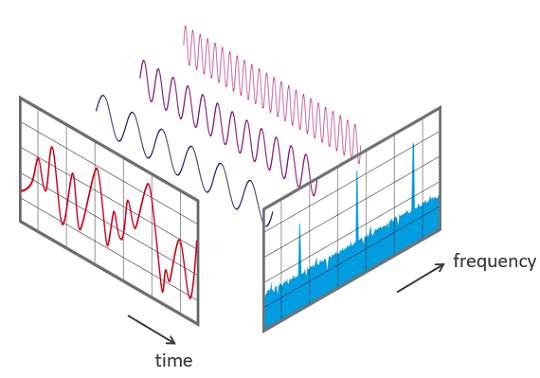
\includegraphics[width=0.4\textwidth]{imgs/time-to-frequency.png}
    \caption{Trasformata di Fourier}
    \label{fig:time_to_frequency}
\end{figure}

La Trasformata di Fourier permette di passare dal dominio temporale, dove il segnale è descritto in funzione del tempo, al dominio della frequenza, offrendo una visione dettagliata delle caratteristiche spettrali del segnale.
Nel contesto pratico, l'analizzatore di spettro trova applicazione in diversi ambiti, tra cui:
\begin{itemize}
    \item \textbf{Diagnostica dei segnali audio:} per identificare distorsioni, rumori o componenti non desiderate;
    \item \textbf{Ingegneria delle telecomunicazioni:} per analizzare la banda occupata da un segnale e ottimizzare la trasmissione;
    \item \textbf{Ingegneria acustica:} per studiare le caratteristiche sonore in ambienti specifici.
\end{itemize}

Un analizzatore di spettro real-time, come quello implementato nel presente progetto, consente di aggiornare continuamente l'analisi del segnale, fornendone una rappresentazione dinamica e interattiva.
Questo è possibile grazie all'utilizzo di algoritmi efficienti per il calcolo della Fast Fourier Transform (FFT) una versione ottimizzata della Trasformata di Fourier discreta (DFT) che riduce significativamente il costo computazionale rispetto all'approccio diretto.
Nella lettura che segue, verrà spiegato ogni aspetto del progetto: dalla scelta e descrizione dei componenti hardware utilizzati, all'implementazione pratica sia della Trasformata di Fourier tramite firmware, sia del rendering grafico sul display OLED, fino alle possibili estensioni future del sistema.
Questo approccio dettagliato permetterà di comprendere non solo il funzionamento dell'analizzatore di spettro, ma anche i principi teorici e pratici che ne stanno alla base.

\section{Teoria dei segnali}

\subsection{Introduzione}
L'obiettivo principale dell'elettronica è il processamento dei segnali.
Un segnale è una funzione matematica che rappresenta la variazione di una grandezza fisica (per esempio la temperatura, la pressione, ...) rispetto ad un'altra quantità (generalmente il tempo).
L'elettronica analogica si concentra sullo studio di segnali continui, detti \textit{segnali analogici}, in termini di tensione e corrente, mentre l'elettronica digitale si concentra sullo studio di segnali discreti, detti \textit{segnali digitali}.
Generalmente i segnali digitali si ottengono partendo da segnali analogici attraverso il processo di \textit{digitalizzazione di un segnale analogico}, riassumibile in tre passi fondamentali: il \textit{campionamento}, la \textit{quantizzazione} e la \textit{codifica}.

\subsection{Conversione analogico-digitale}
Graficamente un segnale analogico è definito sull'intero asse $x$ e può assumere un qualsiasi valore sull'asse $y$, proprio come una funzione $y = f(x)$.
Il \textit{campionamento} è il processo di riduzione di un segnale continuo in un segnale discreto.
In particolare, il segnale discreto è ottenuto considerando i valori del segnale continuo solo a tempo discreto come mostrato in Figura \ref{fig:sampling}.

\begin{figure}[h]
    \centering
    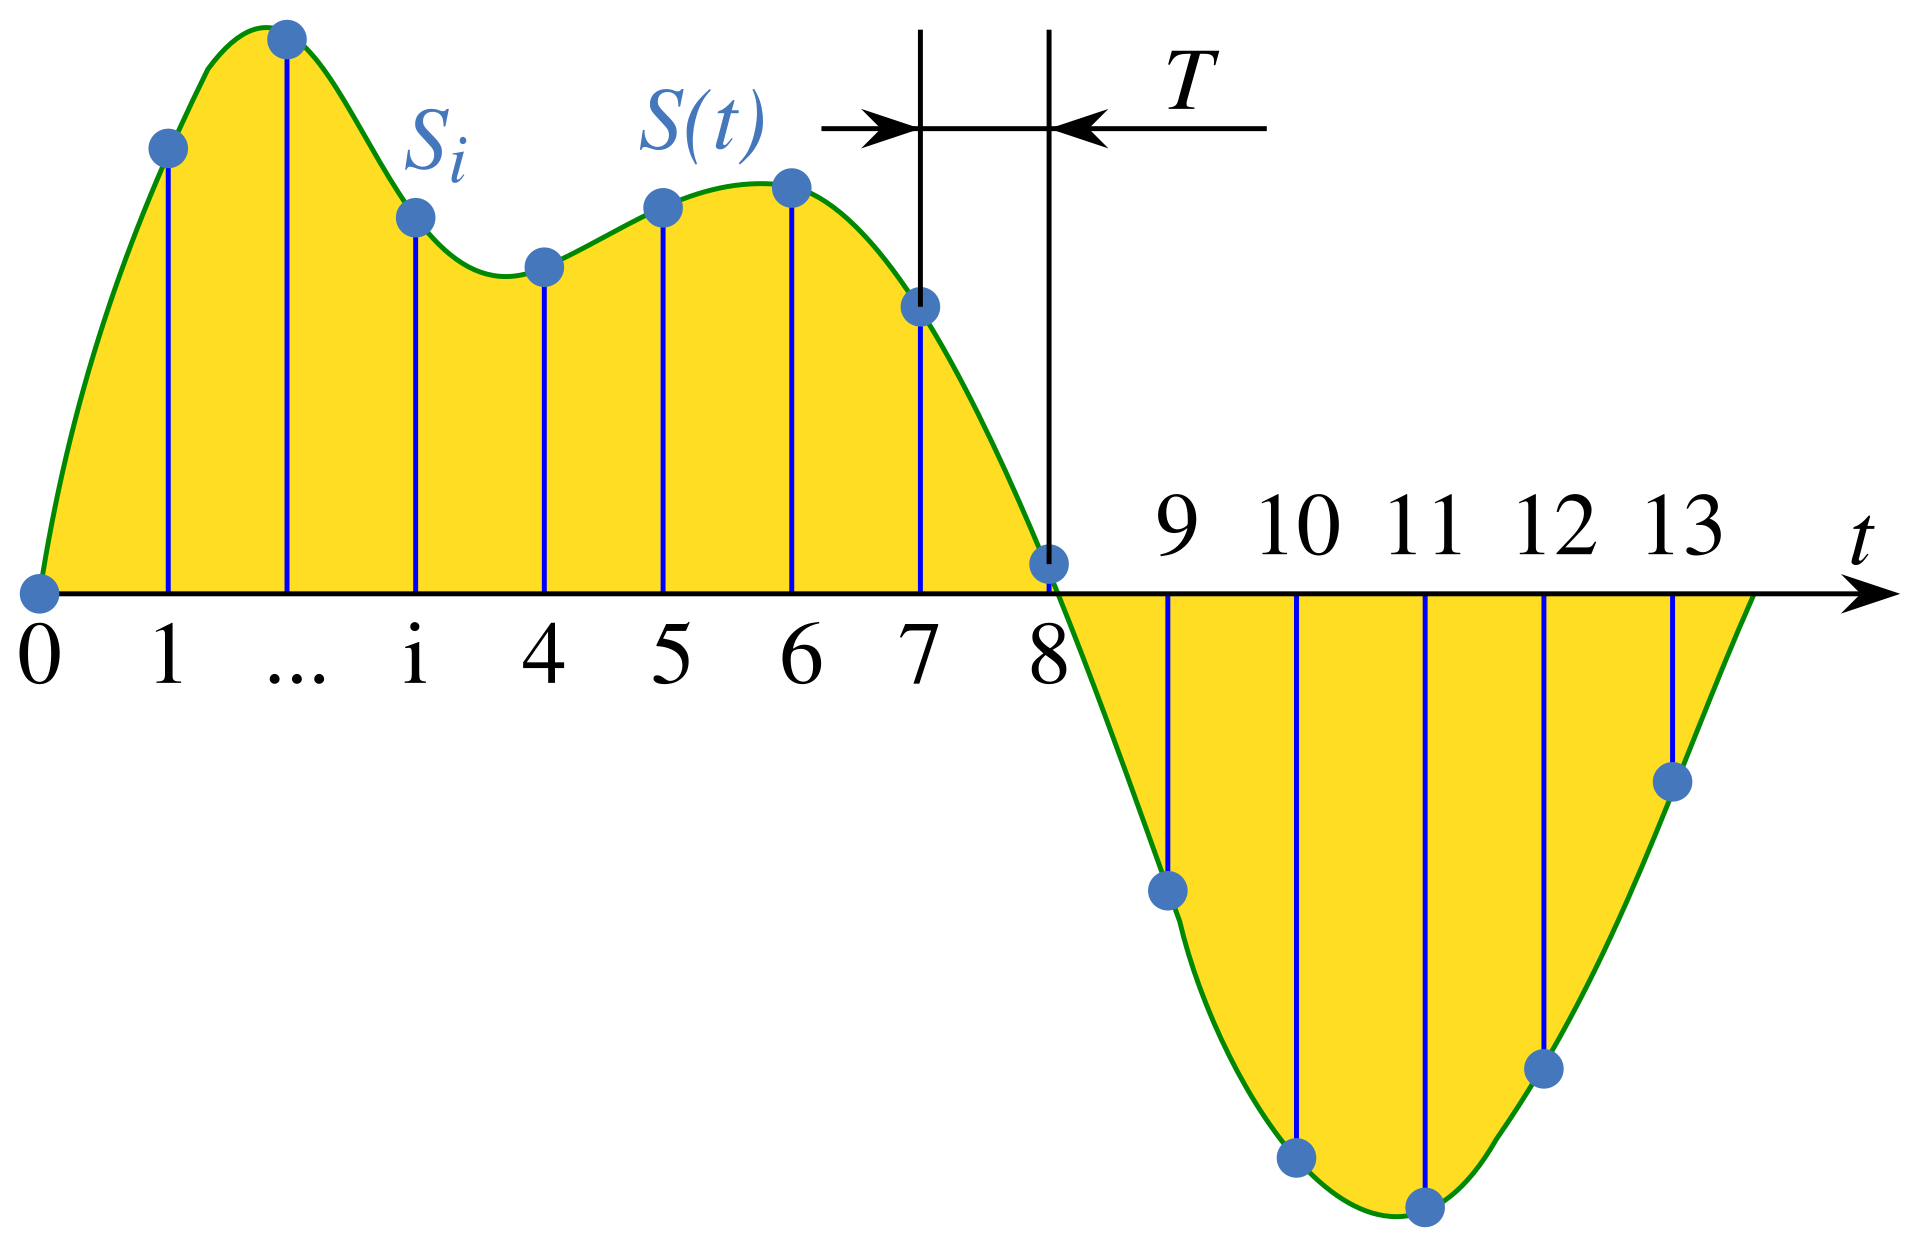
\includegraphics[width=0.35\textwidth]{imgs/Signal_Sampling.png}
    \caption{Campionamento di un segnale analogico}
    \label{fig:sampling}
\end{figure}

Il tempo tra due valori (chiamati anche campioni o \textit{samples}) viene chiamato \textit{tempo di campionamento} e viene indicato con la lettera $T$.
L'inverso del tempo di campionamento definisce la \textit{frequenza di campionamento} $f_s = \frac{1}{T}$.
Tuttavia il campionamento deve rispettare il Teorema di Nyquist-Shannon.

Nello specifico: data la frequenza massima $f_{\text{max}}$ di un segnale analogico, secondo tale teorema la frequenza di campionamento (o \textit{sample rate}) $f_s$ deve essere almeno il doppio della frequenza massima del segnale analogico, cioè $f_s > 2 \cdot f_{\text{max}}$.
Se viene rispettata questa condizione, è possibile -- con l'utilizzo di apposite funzioni interpolatrici -- ricostruire il segnale analogico senza perderne alcuna informazione.
Qualora, al contrario, tale condizione non venga rispettata, il segnale analogico ricostruito sarà distorto (effetto conosciuto con il nome di \textit{aliasing}).
Normalmente, per una buona e fedele ricostruzione del segnale analogico è richiesta una frequenza di campionamento che sia $5 \div 10$ volte maggiore rispetto alla frequenza massima contenuta nel segnale campionato.

Forniamo ora un esempio pratico che chiarisca il concetto di campionamento e il Teorema di Nyquist-Shannon.

Da un segnale analogico e continuo nel tempo preleviamo dei campioni ogni $\Delta t$ secondi\footnote{In questo caso viene usata la notazione $\Delta t$ al posto della notazione $T$ per indicare il tempo di campionamento.}.
Il Teorema di Nyquist-Shannon stabilisce che, dato un segnale analogico $x(t)$ la cui banda di frequenze sia limitata dalla frequenza $f_{\text{max}}$, e dato $n \in \mathbb{Z}$, il segnale $x(t)$ può essere univocamente ricostruito a partire dai suoi campioni $x(n \cdot \Delta t)$ presi a frequenza $f_s = \frac{1}{\Delta t}$ se $f_s > 2 \cdot f_{\text{max}}$ mediante la seguente formula:

\begin{equation}
    x(t) = \sum_{k = -\infty}^{+\infty} x(k \cdot \Delta t) \cdot \text{sinc}\left( \frac{t}{\Delta t} - k \right), \quad \forall t \in \mathbb{R} \nonumber
\end{equation}

dove $\text{sinc}(x) = \frac{\sin(\pi x)}{\pi x}$ è la funzione seno cardinale.

Sulla base di tale formula, utilizzando il seguente codice scritto in linguaggio Python:

\begin{lstlisting}[language=Python,keywords={def, self, class, title, @staticmethod, import, as, arange, sin, pi, figure, subplot, plot, if, xlabel, ylabel, stem, tight_layout, show}]
import numpy as np
import matplotlib.pyplot as plt

AMPLITUDE = 1
F_MAX = 10
T_CONTINUOUS = np.arange(0, 1, 0.01)

class Signal:
    def __init__(self, amplitude, frequency):
        self.amplitude = amplitude
        self.frequency = frequency

    def generate(self, time):
        return self.amplitude * np.sin(2 * np.pi * self.frequency * time)

class SignalPlotter:
    @staticmethod
    def plot_continuous_signal(signal, time):
        x_continuous = signal.generate(time)
        plt.plot(time, x_continuous)
        plt.title(r"$x(t) = \sin(2 \pi f_{\text{max}} t)$")
        plt.xlabel(r"$t$")
        plt.ylabel(r"$x(t)$")

    @staticmethod
    def plot_sampled_signal(subplot_position, caption, signal, sampling_frequency):
        sampling_time = 1 / sampling_frequency
        t_sampled = np.arange(0, 1 + sampling_time, sampling_time)
        x_sampled = signal.generate(t_sampled)
        plt.subplot(2, 2, subplot_position)
        plt.stem(t_sampled, x_sampled)
        plt.title(caption)
        plt.xlabel(r"$t = k \cdot \Delta t$")
        plt.ylabel(r"$x(t) = \sin(2 \pi f_{\text{max}} t)$")

if __name__ == "__main__":
    signal = Signal(amplitude=AMPLITUDE, frequency=F_MAX)

    plt.figure(figsize=(12, 10))
    plt.subplot(2, 2, 1)
    SignalPlotter.plot_continuous_signal(signal, T_CONTINUOUS)

    SignalPlotter.plot_sampled_signal(2, r"$f_s > 2 f_{\text{max}}$", signal, sampling_frequency=4 * F_MAX) # f_s > 2 * f_max
    SignalPlotter.plot_sampled_signal(3, r"$f_s < 2 f_{\text{max}}$", signal, sampling_frequency=10)        # f_s < 2 * f_max
    SignalPlotter.plot_sampled_signal(4, r"$f_s = 2 f_{\text{max}}$", signal, sampling_frequency=2 * F_MAX) # f_s = 2 * f_max

    plt.tight_layout()
    plt.show()
\end{lstlisting}

si ottengono i seguenti grafici:

\begin{figure}[h]
    \centering
    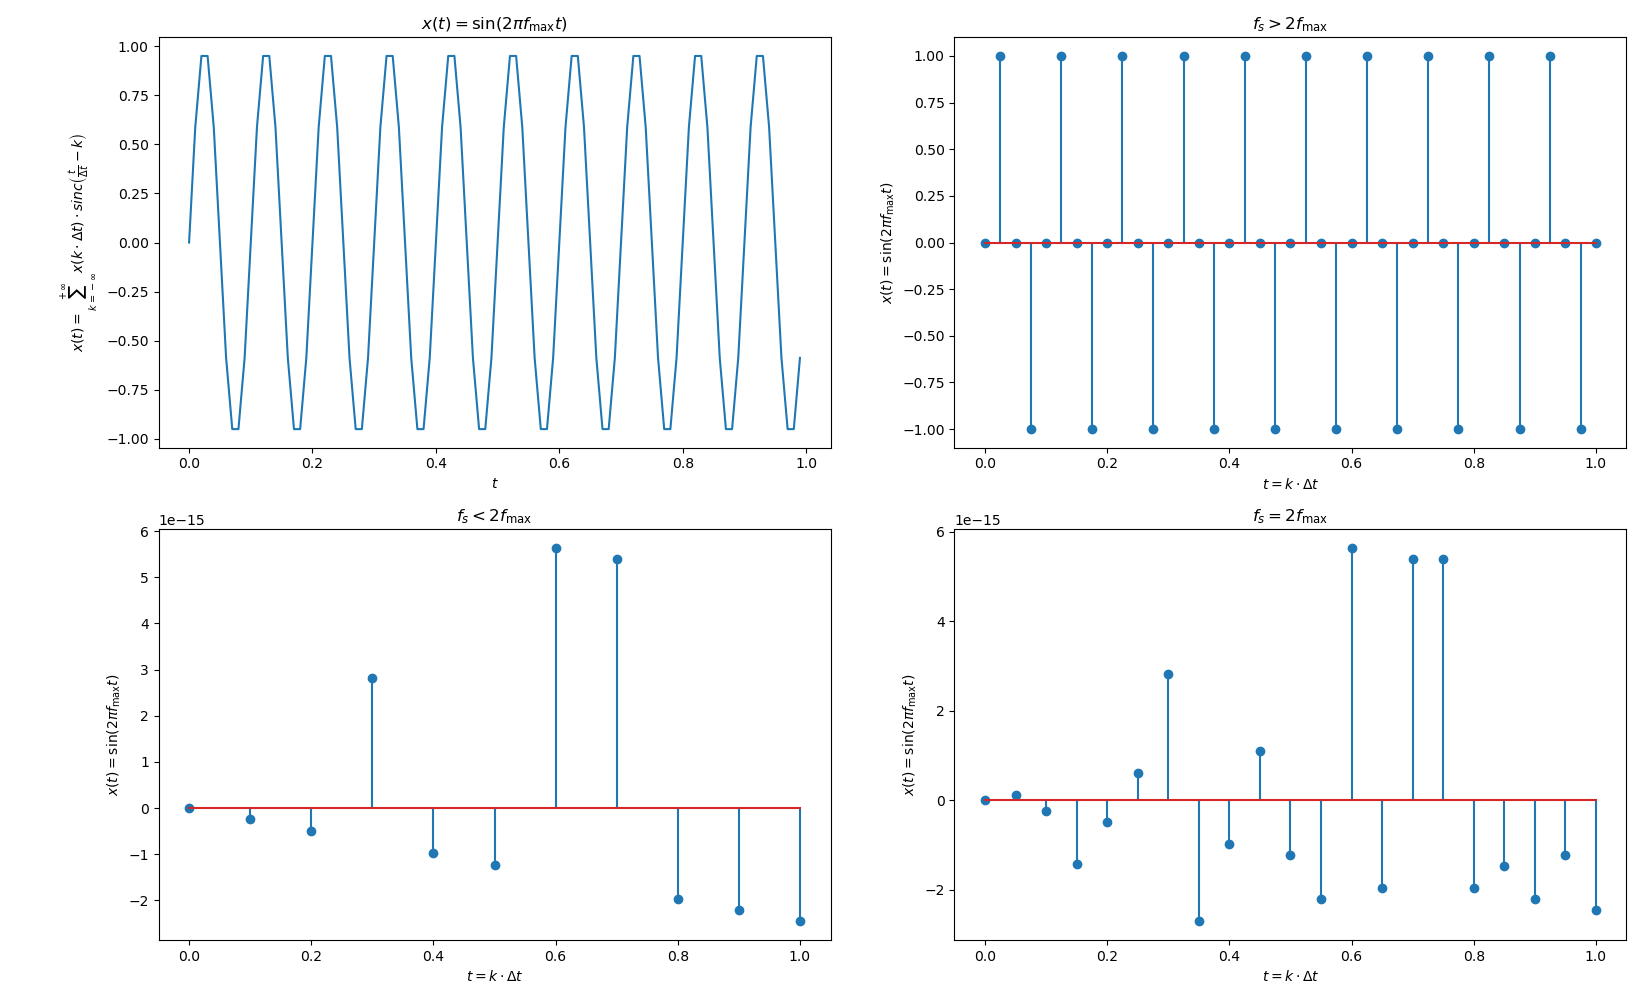
\includegraphics[width=0.8\textwidth]{imgs/nyquist-shannon.png}
    \caption{Campionamento di un segnale analogico}
    \label{fig:Nyquist-Shannon}
\end{figure}

Tale risultato mostra chiaramente come il segnale analogico $x(t) = \sin(2 \pi f_{\text{max}} t)$ può essere ricostruito correttamente solo se la frequenza di campionamento $f_s > 2 \cdot f_{\text{max}}$.
Qualora $f_s \leq 2 \cdot f_{\text{max}}$, si verifica il fenomeno dell'\textit{aliasing}, che comporta una distorsione nel segnale ricostruito.

Introduciamo ora la frequenza di Nyquist definita come $f_N = \frac{f_s}{2}$, dove $f_s$ è la frequenza di campionamento.
Quando un segnale analogico contiene componenti in frequenza che risultino superiori alla frequenza di Nyquist, la loro ricostruzione porta ad un segnale in cui tali componenti risultano \textit{riflesse}, cioè hanno una frequenza specchiata rispetto alla frequenza di Nyquist e rispetto al segnale analogico originale.

Forniamo ora un esempio che illustri chiaramente il concetto di aliasing e fornisca gli strumenti base per mitigarlo o evitarlo.

Se il segnale analogico è una sinusoide con frequenza $f = 12 \text{Hz}$ e la frequenza di campionamento è $f_s = 20 \text{Hz}$, si ottiene $f_r = f_N - (f - f_N) = 8 \text{Hz}$, dove $f_r$ è la frequenza della sinusoide ricostruita.
Poiché la frequenza del segnale $f = 12 \text{Hz}$ è superiore alla frequenza di Nyquist $f_N = 10 \text{Hz}$, durante il campionamento il segnale verrà \textit{aliasato}, cioè la sua frequenza verrà \textit{riflessa} rispetto alla frequenza di Nyquist.
In particolare, il segnale ricostruito avrà una frequenza di $f_r = 8 \text{Hz}$, che è la frequenza specchiata rispetto alla frequenza di Nyquist.

Due sono i possibili approcci finalizzati ad evitare l'aliasing:
\begin{enumerate}
    \item adottare una frequenza di campionamento $f_s$ maggiore, se non si vogliono perdere le informazioni contenute nelle componenti ad alta frequenza del segnale analogico acquisito;
    \item adottare un \textit{filtraggio anti-aliasing} (filtro passa-basso) così da eliminare dal segnale analogico le frequenze maggiori della frequenza di Nyquist del campionatore.
\end{enumerate}

Una volta campionato il segnale, il passo successivo è la \textit{quantizzazione}, che consiste nel mappare i valori campionati su un discreto insieme di valori.
In particolare, l'asse $y$ del segnale analogico viene diviso in $n$ livelli, chiamati \textit{livelli di quantizzazione}.
Ogni valore campionato viene quindi mappato sul livello di quantizzazione più vicino, generando un segnale discreto.
Il risultato si può visualizzare in Figura \ref{fig:quantization}, dove viene raffigurata una griglia che combina campionamento e quantizzazione.

\begin{figure}[h]
    \centering
    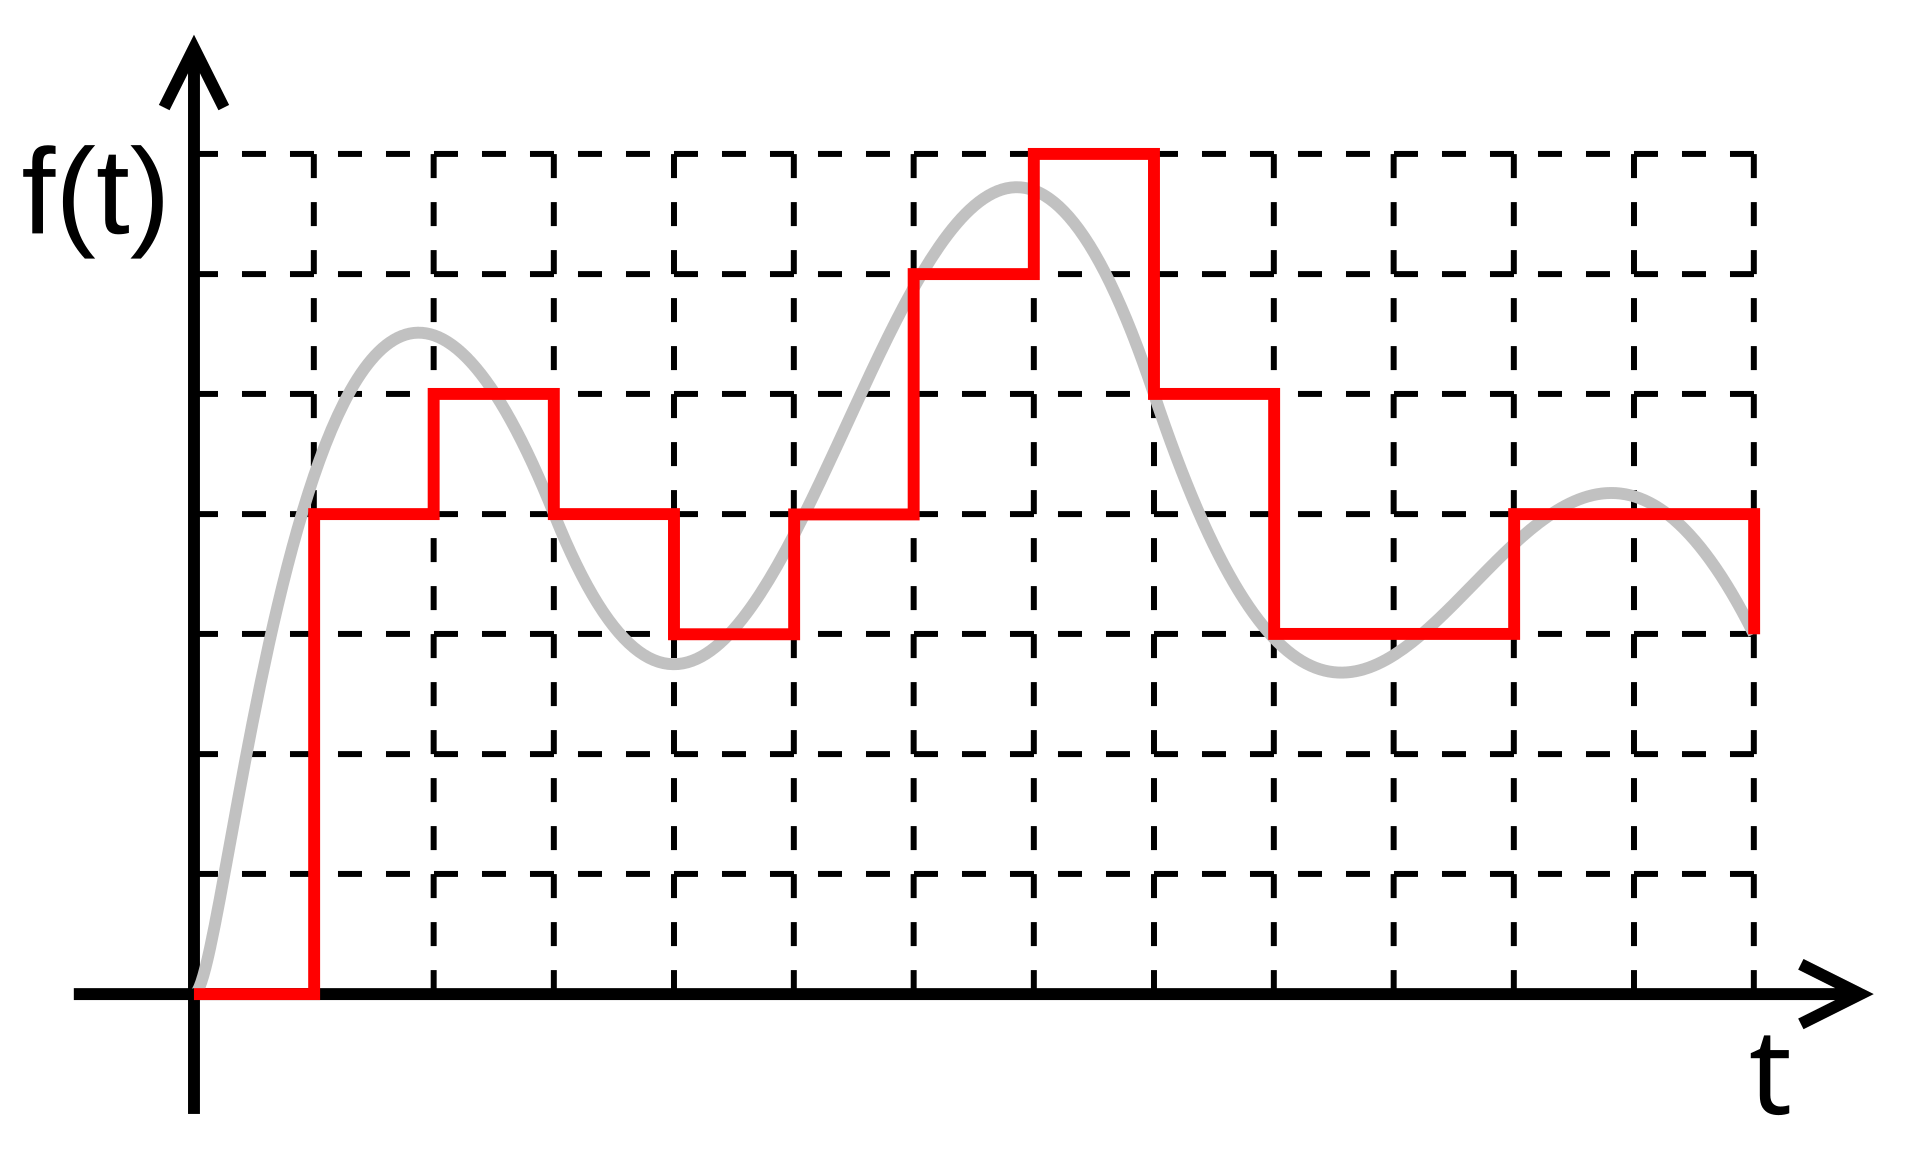
\includegraphics[width=0.5\textwidth]{imgs/Quantization.png}
    \caption{Quantizzazione di un segnale analogico}
    \label{fig:quantization}
\end{figure}

Come per il campionamento, ove l'errore dà luogo all'\textit{aliasing}, anche per la quantizzazione si può parlare di errore, che consiste nella differenza tra il valore campionato e il valore quantizzato.
Per ridurre gli effetti dell'\textit{errore di quantizzazione}, è possibile aumentarne il numero di livelli, riducendo la distanza tra questi.
In particolare, gli $n$ livelli di quantizzazione sono legati ai bit che vengono utilizzati per rappresentare il segnale digitale tramite la formula $n = 2^k$, dove $k$ è il numero di bit.
Più bit si usano, migliore sarà il rapporto segnale-rumore (SNR).
Ad ogni aumento di $1$ bit si ha un incremento di circa $6 \text{dB}$ dell'SNR.

Perchè proprio $6 \text{dB}$? Supponiamo di avere un segnale digitale che può essere rappresentato da un certo numero di livelli discreti.
Se aumentiamo di $1$ bit, il numero di livelli possibili e l'ampiezza del segnale raddoppiano (infatti $n = 2^{k + 1} = 2 \cdot 2^k$).
La variazione in decibel è data dalla formula:

\begin{equation}
    \Delta L = 10 \cdot \log_{10} \left( \frac{P_1}{P_0} \right) = 10 \cdot \log_{10} \left( \frac{\frac{V_1^2}{R}}{\frac{V_0^2}{R}} \right) = 20 \cdot \log_{10} \left( \frac{V_1}{V_0} \right) \nonumber
\end{equation}

dove $P_1$ e $P_0$ sono le potenze del segnale in uscita e in ingresso, $V_1$ e $V_0$ sono le tensioni del segnale in uscita e in ingresso ed infine $R$ è la resistenza di carico.
Considerando un generico segnale sinusoidale di tensione elettrica nella seguente forma:

\begin{equation}
    v(t) = V_0 \cdot \sin(2 \pi f t) \nonumber
\end{equation}

dove $V_0$ è l'ampiezza del segnale, $f$ è la frequenza e $t$ è il tempo, sapendo che $V_1 = 2 \cdot V_0$ (perchè con $k + 1$ bit raddoppia l'ampiezza) otterremo il seguente risultato:

\begin{equation}
    \Delta L \approx 6.02 \ \text{dB} \nonumber
\end{equation}

\subsection{Sistemi digitali}
In generale, un sistema elettronico è composto dai seguenti elementi:

\begin{figure}[h]
    \centering
    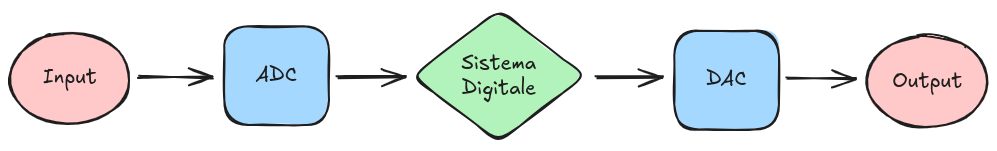
\includegraphics[width=1.0\textwidth]{imgs/electronics-system-elements.png}
    \caption{Elementi di un sistema elettronico.}
    \label{fig:system}
\end{figure}

dove:

\begin{itemize}
    \item l'\textit{Input} è il segnale analogico in ingresso al sistema;
    \item l'ADC (\textit{Analog-to-Digital Converter}) è il convertitore analogico-digitale che trasforma il segnale analogico in un segnale digitale;
    \item il \textit{sistema digitale} è il sistema che elabora il segnale digitale che può essere un microprocessore, un microcontrollore, un FPGA, un DSP, un ASIC (per esempio una GPU);
    \item il DAC (\textit{Digital-to-Analog Converter}) è il convertitore digitale-analogico che trasforma il segnale digitale in un segnale analogico;
    \item l'\textit{Output} è il segnale analogico in uscita dal sistema.
\end{itemize}

Tuttavia, ai fini del presente progetto, occorre considerare un sistema elettronico meno complesso rispetto a quello rappresentato in Figura \ref{fig:system}, riconducibile al seguente schema:

\begin{figure}[h]
    \centering
    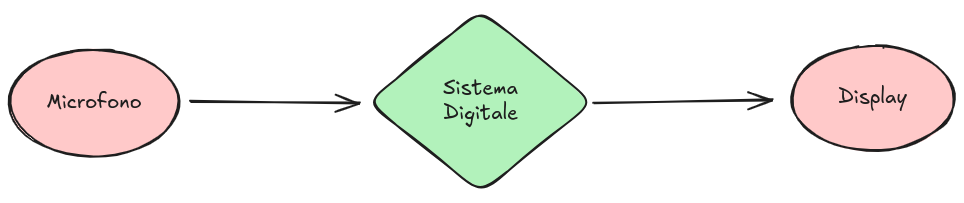
\includegraphics[width=0.75\textwidth]{imgs/electronics-system-elements-fft.png}
    \caption{Elementi del sistema elettronico per l'analizzatore di spettro.}
    \label{fig:easy_system}
\end{figure}

Come si può notare, l'ADC non è presente perchè esso è già integrato all'interno del sistema digitale.
Inoltre, non c'è la necessità di ricostruire il segnale analogico in uscita (quindi l'onda sonora acquisita dal microfono) ma solo di visualizzarlo su un display, utilizzando la Trasformata di Fourier.

\subsection{Acquisizione del segnale audio}\label{sec:acquisition}
Per acquisire il segnale audio, è necessario utilizzare un microfono che trasformi le onde sonore in segnali elettrici.

Iniziamo col mostrare come è possibile acquisire il segnale audio attraverso il linguaggio C\texttt{++} per dispositivi embedded.
A tal fine utilizziamo la funzione \lstinlinebg{loop()} e, al suo interno, la funzione \lstinlinebg{analogRead()} che leggerà il valore del segnale audio acquisito dal microfono.
Tale lettura va eseguita ogni $T = \frac{1}{f_s}$ microsecondi, avendo cura di impostare una frequenza di campionamento $f_s$ adeguata al fine di evitare l'aliasing.

Come verrà spiegato più avanti\footnote{Vedi sezione \ref{sec:code}.}, utilizziamo la variabile \lstinlinebg{engine.samplingPeriod}, che rappresenta il tempo di campionamento espresso in microsecondi.

Il codice che ne risulta è il seguente:

\begin{lstlisting}[language=C++,keywords={const, uint8_t, if, for, void, Serial, begin, uint16_t, analogRead, println, uint32_t, micros, pinMode, INPUT}]
const uint32_t interval = engine.samplingPeriod;
uint32_t lastUpdate = 0;

void setup() {
    pinMode(AUDIO_IN_PIN, INPUT);
    lastUpdate = micros();
}

void loop() {
    // Acquisition of audio samples
    if (micros() - lastUpdate >= interval) {
        lastUpdate = micros();
        for (uint8_t i = 0; i < SAMPLES; ++i) {
            uint16_t sample = analogRead(AUDIO_IN_PIN);
            engine.re[i] = sample;
            engine.im[i] = 0.0;
        }

        // ...
    }
}
\end{lstlisting}

si noti la presenza delle variabili \lstinlinebg{engine.re[i]} e \lstinlinebg{engine.im[i]}, che rappresentano rispettivamente la parte reale e la parte immaginaria del segnale acquisito, distinzione dovuta al fatto che la Trasformata di Fourier è una trasformata complessa.
Si noti, infine, che grazie alla condizione \lstinlinebg{if (micros() - lastUpdate >= interval)} siamo in grado di acquisire il segnale audio ad una adeguata frequenza di campionamento $f_s$.

\subsection{Analisi del segnale audio}
Una volta acquisito dal microfono\footnote{Si fa notare che per esigenze di sintesi sono stati volutamente omessi i dettagli sui componenti hardware utilizzati, dando per scontata l'acquisizione del segnale tramite microfono. Per i dettagli sul microfono utilizzato si rimanda alla sezione \ref{sec:design}.} il segnale audio, il passo successivo è la sua analisi.
Fondamentale è la preparazione del segnale per per potergli applicare la Trasformata di Fourier (analisi spettrale).

\subsubsection{Filtraggio del segnale}\label{sec:filtering}
Esistono due tipologie principali di filtraggio: il \textit{filtraggio hardware} e il \textit{filtraggio software}.
Entrambe le tecniche hanno vantaggi e svantaggi.
Il filtraggio hardware è generalmente più efficiente e veloce, ma richiede modifiche all'hardware e può essere meno flessibile.
Il filtraggio software è più flessibile e può essere facilmente modificato, ma richiede più risorse computazionali e può introdurre ritardi nel segnale.
Il filtraggio hardware ci permette di utilizzare un filtro passa-basso analogico per eliminare le frequenze superiori alla frequenza di Nyquist.
A tal fine si possono utilizzare componenti passivi come resistenze, condensatori e induttori, oppure componenti attivi come amplificatori operazionali.
In particolare, indipendentemente dal tipo di componenti che scegliamo di utilizzare\footnote{Questa affermazione, che è assolutamente valida per i circuiti elettronici che utilizzano unicamente componenti passivi, lo è anche nel caso di circuiti che utilizzano componenti attivi. Ciò in quanto questi ultimi dovranno, a loro volta, fare uso di componenti passivi per rendere il circuito stabile e assicurare un corretto funzionamento dello stesso.}, la realizzazione del filtro dipende dal dimensionamento dei componenti $R$ e $C$, con i quali si ottiene un filtro passa-basso con una frequenza di taglio $f_t$ pari alla frequenza di Nyquist, ovvero tale da rispettare la seguente relazione:

\begin{equation}
    f_t = \frac{1}{2 \pi R C} = f_N \nonumber
\end{equation}

dove $R$ è la resistenza e $C$ è il condensatore.

Per quanto riguarda il filtraggio software, al fine di eliminare le frequenze superiori alla frequenza di Nyquist, si può utilizzare un filtro digitale come il filtro FIR (\textit{Finite Impulse Response}) o il filtro IIR (\textit{Infinite Impulse Response}).
In particolare, un semplice filtro IIR può essere implementato con la seguente equazione ricorsiva:

\begin{equation}
    y[n] = \alpha \cdot x[n] + (1 - \alpha) \cdot y[n - 1] \nonumber
\end{equation}

dove $y[n]$ è l'uscita del filtro al campione $n$-esimo, $x[n]$ è l'ingresso del filtro e $\alpha$ è un parametro che determina la frequenza di taglio del filtro ed è definito come:

\begin{equation}
    \alpha = \frac{T}{T + \tau} \nonumber
\end{equation}

dove $T$ è il tempo di campionamento e $\tau$ è la costante di tempo del filtro che è correlata alla frequenza di taglio.

Per questo progetto, si è scelto di utilizzare un filtraggio software per la sua flessibilità e facilità di implementazione.
A tal proposito, si riporta di seguito, l'implementazione di un filtro IIR passa-basso in linguaggio C\texttt{++} per dispositivi embedded:

\begin{lstlisting}[language=C++,keywords={const, uint8_t, float, this, return, uint16_t, analogRead, println, delay}]
float EngineFFT::antiAliasingLowPassFilter(uint16_t sample) {
    // Normalize the sample value to a range between 0 and 1
    float currentValue = sample / ((1 << ADC_RESOLUTION) - 1.0f);
    
    // IIR Low-Pass Filter
    float filteredValue = alpha * currentValue + (1.0f - alpha) * this->lastFilteredValue;
    this->lastFilteredValue = filteredValue;
    
    return filteredValue;
}
\end{lstlisting}

dove \lstinlinebg{alpha} è il parametro che determina la frequenza di taglio del filtro IIR, mentre \lstinlinebg{this->lastFilteredValue} è il valore del campione precedente.
Per utilizzare il filtro IIR passa-basso è sufficiente chiamare la funzione \lstinlinebg{engine.antiAliasingLowPassFilter(sample)} passando come parametro il valore del campione acquisito attraverso il microfono.
Pertanto, il codice mostrato nella sezione \ref{sec:acquisition} andrà modificato come segue:

\begin{lstlisting}[language=C++,keywords={antiAliasingLowPassFilter, const, uint8_t, if, for, void, Serial, begin, uint16_t, analogRead, println, uint32_t, micros, pinMode, INPUT}]
const uint32_t interval = engine.samplingPeriod;
uint32_t lastUpdate = 0;

void setup() {
    pinMode(AUDIO_IN_PIN, INPUT);
    lastUpdate = micros();
}

void loop() {
    // Acquisition of audio samples
    if (micros() - lastUpdate >= interval) {
        lastUpdate = micros();
        for (uint8_t i = 0; i < SAMPLES; ++i) {
            uint16_t sample = analogRead(AUDIO_IN_PIN);
            engine.re[i] = engine.antiAliasingLowPassFilter(sample);
            engine.im[i] = 0.0;
        }
     
        // ...
    }
}
\end{lstlisting}

\subsubsection{Rimozione del DC offset}\label{sec:dc_offset}
Un ulteriore passo fondamentale riguarda la rimozione del \textit{DC offset} dal segnale audio.
Il DC offset è una componente costante del segnale audio (Figura \ref{fig:dc_offset}) che può essere causata da vari fattori, quali rumore elettrico, interferenze, errori di calibrazione o errori di acquisizione.
La presenza del DC offset può influenzare l'analisi spettrale del segnale audio, introducendo errori e distorsioni.
Sostanzialmente si tratta di una traslazione del segnale audio lungo l'asse verticale, che può essere facilmente identificata visualizzando il segnale nel dominio del tempo.

\begin{figure}[h]
    \centering
    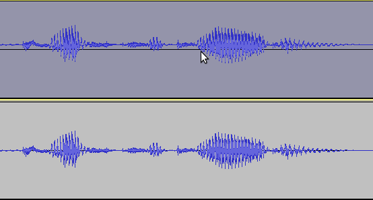
\includegraphics[width=0.35\textwidth]{imgs/dc_offset-audacity.png}
    \caption{DC offset nel programma Audacity.}
    \label{fig:dc_offset}
\end{figure}

È necessario, pertanto, rimuovere il DC offset dal segnale audio prima di procedere con l'analisi spettrale.
A tal fine si può utilizzare una funzione che sottrae la media del segnale dal segnale stesso.
In particolare, la media del segnale può essere calcolata utilizzando una semplice media aritmetica:

\begin{equation}
    \mu = \frac{1}{N} \sum_{n = 0}^{N - 1} x[n] \nonumber
\end{equation}

dove $x[n]$ è il campione $n$-esimo del segnale audio e $N$ è il numero totale di campioni.
Una volta calcolata la media del segnale, è possibile rimuovere il DC offset sottraendo la media da ciascun campione:

\begin{equation}
    y[n] = x[n] - \mu \nonumber
\end{equation}

dove $y[n]$ è il campione $n$-esimo del segnale audio senza il DC offset.
Ne deriva la seguente funzione in linguaggio C\texttt{++} per dispositivi embedded:

\begin{lstlisting}[language=C++,keywords={void, double, float, this, uint16_t, this, for}]
void EngineFFT::removeDC(void) {
    double mean = 0.0;
    for (uint16_t i = 0; i < SAMPLES; ++i) {
        mean += this->re[i];
    }
    mean /= SAMPLES;
    for (uint16_t i = 0; i < SAMPLES; ++i) {
        this->re[i] -= mean;
    }
}
\end{lstlisting}

che implementa la rimozione del DC offset dal segnale audio acquisito.

\subsubsection{Windowing del segnale}\label{sec:windowing}
Ultimo step per concludere la preparazione del segnale audio per l'analisi spettrale è il \textit{windowing}.
Nell'elaborazione numerica dei segnali, una \textit{funzione finestra} è una funzione che, al di fuori di un certo intervallo, vale zero.
Quando un'altra funzione è moltiplicata per una funzione finestra, anche il prodotto assume valori nulli al di fuori dell'intervallo: tutto ciò che resta è la \textquotedblleft vista\textquotedblright \ attraverso la finestra.
Esisitono vari tipi di funzioni finestra, tra cui la \textit{finestra rettangolare}, la \textit{finestra di Hann}, la \textit{finestra di Hamming} e la \textit{finestra di Blackman}.

\begin{figure}[h]
    \centering
    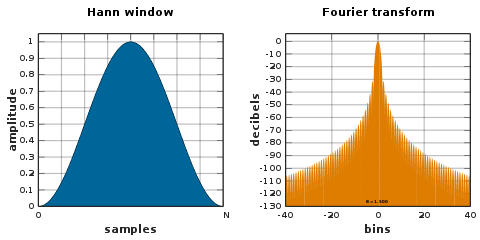
\includegraphics[width=0.5\textwidth]{imgs/Window_function_Hann.png}
    \caption{Finestra di Hann applicata al segnale audio.}
    \label{fig:hann_window}
\end{figure}

L'obiettivo principale dell'utilizzo di una funzione finestra è quello di minimizzare l'\textit{effetto di leakage} nelle frequenze risultanti dalla Trasformata di Fourier.
L'effetto di leakage si verifica quando il segnale campionato non corrisponde esattamente a un numero intero di cicli della frequenza che si sta cercando di analizzare.
Questo porta a una distorsione nei risultati, causando la diffusione dell'energia del segnale su frequenze adiacenti.
In altre parole, se la frequenza del segnale non è esattamente un multiplo intero della frequenza di campionamento, il segnale apparirà \textit{diluito} in frequenza, rendendo difficile identificare con precisione la sua frequenza e ampiezza nello spettro risultante.
Per questo progetto si è scelta una delle finestre più comuni e ampiamente utilizzate in applicazioni audio, la \textit{finestra di Hann}, definita come:

\begin{equation}
    w[n] = 0.5 \cdot \left [ 1 - \cos \left( \frac{2 \pi n}{N - 1} \right) \right ] \nonumber
\end{equation}

dove $w[n]$ è il valore della finestra di Hann al campione $n$-esimo ed $N$ è il numero totale di campioni.
Il risultato dell'applicazione della finestra di Hann al segnale audio è mostrato in Figura \ref{fig:hann_window}.

Quello che segue è il codice per la fuzione di windowing in linguaggio C\texttt{++} per dispositivi embedded:

\begin{lstlisting}[language=C++,keywords={void, double, float, this, uint16_t, this, for, cos, TWO_PI}]
void EngineFFT::windowing(void) {
    double samplesMinusOne = SAMPLES - 1.0;
    for (uint16_t i = 0; i < (SAMPLES >> 1); ++i) {
        double ratio = i / samplesMinusOne;
    
        // Hann Window factor
        double weighingFactor = 0.5 * (1.0 - cos(TWO_PI * ratio));
    
        // Applying Hann Window to samples
        this->re[i] *= weighingFactor;
        this->re[SAMPLES - (i + 1)] *= weighingFactor;
    }
}
\end{lstlisting}

\subsection{Trasformata di Fourier (DFT e FFT)}\label{sec:fft}
La Trasformata di Fourier discreta (DFT) è uno strumento matematico fondamentale per analizzare segnali nel dominio del tempo trasformandoli in segnali nel dominio della frequenza.
Questo approccio permette di rappresentare un segnale come somma di sinusoidi (o esponenziali complessi) di diverse frequenze, ampiezze e fasi.
La DFT di una sequenza di $N$ campioni $x[n]$ è definita come:
\begin{equation}
    X[k] = \sum_{n = 0}^{N - 1} x[n] \cdot e^{-j \frac{2 \pi k n}{N}}, \quad k = 0, 1, \ldots, N - 1 \nonumber
\end{equation}
dove $X[k]$ è il $k$-esimo campione della DFT, $x[n]$ è l'$n$-esimo campione del segnale in ingresso, $j$ è l'unità immaginaria, $N$ è il numero totale di campioni ed infine $e^{-j \frac{2 \pi k n}{N}}$ è l'esponenziale complesso.

In termini di informatica teorica, la definizione della DFT, ha un elevato costo computazionale che la rende inefficiente per dispositivi embedded con risorse limitate.

Dal punto di vista puramente pratico, implementare la definizione della funzione \lstinlinebg{dft()} in linguaggio C, comporta un codice simile al seguente:
\begin{lstlisting}[language=C,keywords={void, complex, float, size_t, for, double, cexp, I, M_PI}]
void dft(float in[], float complex out[], size_t N) {
    for (size_t k = 0; k < N; ++k) {
        out[k] = 0;
        for (size_t n = 0; n < N; ++n) {
            double angle = -2.0 * M_PI * k * n / N;
            out[k] += in[n] * cexp(angle * I);
        }
    }
}
\end{lstlisting}
dove, per ogni campione $k$-esimo della DFT, si calcola la somma di tutti i campioni $n$-esimi del segnale moltiplicati per l'esponenziale complesso.
Ciò rende il costo computazionale della DFT pari a $O(N^2)$.
Inoltre, poichè nei dispositivi embedded non esiste il tipo di dato \lstinlinebg{complex}, occorre gestire separatamente la parte reale e la parte immaginaria del segnale.
Anche per questo motivo, è stata introdotta la \textit{Fast Fourier Transform} (FFT) un algoritmo efficiente per calcolare la DFT con un costo computazionale pari a $O(N \text{log}_2 N)$.

L'algoritmo FFT è stato inventato da Cooley e Tukey nel $1965$ e da allora è diventato uno degli algoritmi più importanti e ampiamente utilizzati in vari campi, tra cui l'elaborazione numerica dei segnali, la teoria dei numeri, la crittografia, e molti altri.
Per questo motivo, nel nostro progetto, si è scelto di utilizzare l'algoritmo di Cooley-Tukey, in particolare la versione \textit{radix-2}, che è la più comune e ampiamente utilizzata.
Questo algoritmo si basa sulla tecnica del \textit{divide et impera}, suddividendo ricorsivamente il segnale in ingresso in sottoinsiemi di dimensioni pari e dispari, e sulle \textit{butterfly operations}.

A questo punto è necessario introdurre il concetto di \textit{bit reversal}, tecnica utilizzata per riordinare i campioni del segnale in ingresso.

\subsubsection{Bit Reversal Algorithm}
L'algoritmo di \textit{bit reversal} è una tecnica che permette di separare i campioni con indice dispari dai campioni con indice pari, cosicchè nella prima metà (da $0$ a $\frac{N}{2} - 1$) si trovino i campioni con indice pari e nella seconda metà (da $\frac{N}{2}$ a $N - 1$) si trovino i campioni con indice dispari\footnote{dove con $N$ si indica il numero di campioni.}.

Per implementare tale algoritmo in linguaggio C\texttt{++} per dispositivi embedded, si può utilizzare il seguente codice:
\begin{lstlisting}[language=C++, keywords={void, uint16_t, while, for, if, this}]
uint16_t j = 0;
for (uint16_t i = 0; i < (SAMPLES - 1); ++i) {
    if (i < j) this->swap(&this->re[i], &this->re[j]);
    uint16_t k = SAMPLES >> 1;
    while (k <= j) {
        j -= k;
        k >>= 1;
    }
    j += k;
}
\end{lstlisting}
Trattandosi di un singolo ciclo \lstinlinebg{for}, questo algoritmo può essere già implementato all'interno della funzione \lstinlinebg{fft()}\footnote{Per maggiori informazioni riguardo l'organizzazione del codice sorgente del progetto è possibile consultare la sezione \ref{sec:code}.} senza creare una funzione appositamente dedicata.
Ciò non vale per la funzione \lstinlinebg{swap()} che necessita di implementazione separata:
\begin{lstlisting}[language=C++, keywords={void, double}]
void EngineFFT::swap(double *x, double *y) {
    double temp = *x;
    *x = *y;
    *y = temp;
}
\end{lstlisting}

\subsubsection{Algoritmo di Cooley-Tukey}
In via preliminare definiamo i concetti di \textit{butterfly operation} e \textit{twiddle factor}.

La \textit{butterfly operation} è una tecnica utilizzata nell'algoritmo FFT per calcolare la DFT di un segnale diviso in due parti (pari e dispari) definita come segue:

\begin{equation}
    \begin{cases}
        X[k] = E[k] + W_N^k \cdot O[k] \\
        X[k + \frac{N}{2}] = E[k] - W_N^k \cdot O[k]
    \end{cases} \label{eq:butterfly}
\end{equation}

dove $X[k]$ è il $k$-esimo campione della DFT, $X[k + \frac{N}{2}]$ è il $k + \frac{N}{2}$-esimo campione della DFT, $E[k]$ è il $k$-esimo campione della DFT della parte pari del segnale, $O[k]$ è il $k$-esimo campione della DFT della parte dispari del segnale, $W_N^k$ è il \textit{twiddle factor} definito come $W_N^k = e^{-j \frac{2 \pi k}{N}}$, $k = 0, 1, \ldots, 7$ ed $N$ è il numero totale di campioni.
\noindent\\ Il \textit{twiddle factor} è un fattore complesso che ruota il segnale di un certo angolo, così da calcolare la DFT di un segnale diviso in due parti.
Consideriamo un numero totale di campioni pari a $N = 8$\footnote{Consideriamo un numero abbastanza piccolo per far comprendere al meglio il concetto. Infatti, nella pratica il numero di campioni è tendenzialmente $N \geq 128$.}.
In questo caso, il twiddle factor $W_8^k$ è definito come segue:

\begin{equation}
    W_8^k = e^{-j \frac{\pi k}{4}} \nonumber
\end{equation}

Trattandosi di un fattore complesso, si otterà il piano di Gauss mostrato in Figura \ref{fig:twiddle_factor}.

\begin{figure}[h!]
    \centering
    \begin{tikzpicture}[scale=1.5]
        % Draw the unit circle
        \draw[thick] (0,0) circle(1);

        % Extend and label the axes
        \draw[->] (-1.5,0) -- (1.5,0) node[right] {$\operatorname{Re}$};
        \draw[->] (0,-1.5) -- (0,1.5) node[above] {$\operatorname{Im}$};

        % Divide the circle into 8 parts (like a pie chart)
        \foreach \i in {0,...,7} {
            \pgfmathsetmacro{\angle}{360/8 * \i}
            \draw[thin,dashed] (0,0) -- ({cos(\angle)},{sin(\angle)});
        }

        % Add the twiddle factors
        \foreach \i in {0,...,7} {
            \pgfmathsetmacro{\angle}{-360/8 * \i} % Negative angle for clockwise
            \pgfmathsetmacro{\x}{cos(\angle)}
            \pgfmathsetmacro{\y}{sin(\angle)}

            % Draw the twiddle factors as points
            \node[circle,fill,inner sep=1pt] at (\x,\y) {};

            % Adjust label positions for specific angles
            \ifnum\i=0
                \node[anchor=north] at (\x*1.3,\y*1.3) {$W_8^{\i}$}; % 0 degrees
            \else\ifnum\i=2
                \node[anchor=east] at (\x*1.3,\y*1.3) {$W_8^{\i}$}; % 180 degrees
            \else\ifnum\i=4
                \node[anchor=south] at (\x*1.3,\y*1.3) {$W_8^{\i}$}; % 90 degrees
            \else\ifnum\i=6
                \node[anchor=west] at (\x*1.3,\y*1.3) {$W_8^{\i}$}; % 270 degrees
            \else
                \node[anchor=center,scale=0.8] at (\x*1.3,\y*1.3) {$W_8^{\i}$};
            \fi\fi\fi\fi
        }
    \end{tikzpicture}
    \caption{Rappresentazione dei twiddle factors $W_8^k$ con $k = 0, \dots, 7$.}
    \label{fig:twiddle_factor}
\end{figure}

È evidente come i twiddle factors $W_8^k$ siano disposti uniformemente sulla circonferenza unitaria del piano complesso, con un angolo di $\frac{\pi}{4}$ tra ciascun fattore.
Pertanto è possibile ricavare i seguenti legami fondamentali, validi anche nel caso in cui il numero di campioni è $N$:

\begin{equation}
    W_8^0 = -W_8^4, \quad W_8^1 = -W_8^5, \quad W_8^2 = -W_8^6, \quad W_8^3 = -W_8^7 \nonumber
\end{equation}

Facendo riferimento alla Figura \ref{fig:butterfly} e alle relazioni \eqref{eq:butterfly} si può notare come i twiddle factors $W_8^k$ vengano utilizzati per calcolare la DFT di un segnale diviso in due parti validando le relazioni sopra citate.

Tornando alle \textit{butterfly operations}, una volta che il segnale è stato riordinato tramite l'algoritmo di \textit{bit reversal}, possiamo applicare l'algoritmo FFT per calcolare la DFT di tale segnale.
In particolare, facciamo riferimento alla sottostante Figura \ref{fig:butterfly}, la quale rappresenta le \textit{butterfly operations} per un segnale con $N = 8$ campioni.
Come si può notare, in input ci sono i campioni $x[0], \dots, x[7]$, opportunamente riordinati dal \textit{bit reversal}, mentre in output ci sono i campioni $X[0], \dots, X[7]$ che rappresentano la DFT del segnale in ingresso.
Sia alla prima metà che alla seconda metà dei campioni viene applicata la DFT (anche detta \textit{sub-DFT}) la quale, lavorando con un numero di campioni più piccolo rispetto al totale dei campioni, permette di ridurre il costo computazionale.

\begin{figure}[h]
    \centering
    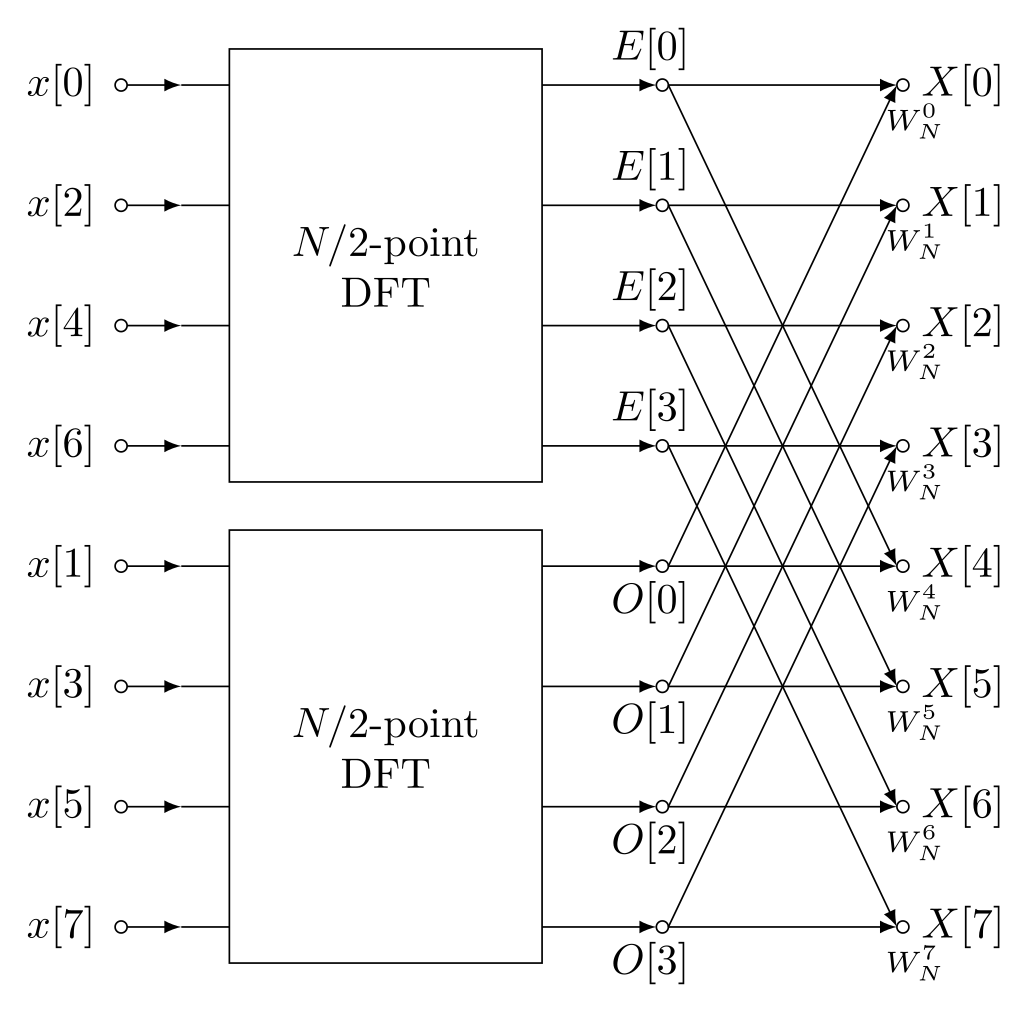
\includegraphics[width=0.4\textwidth]{imgs/DIT-FFT-butterfly.png}
    \caption{Butterfly operations per un segnale con $N = 8$ campioni.}
    \label{fig:butterfly}
\end{figure}

Terminate le \textit{sub-DFT}, si ottegono $4$ campioni $E[0], \dots, E[3]$ e $4$ campioni $O[0], \dots, O[3]$ (rispettivamente \textit{even} e \textit{odd}).
In nostro ragionamento vale nel momento in cui ci troviamo ad uno specifico livello\footnote{Con il termine livello, si intende la grandezza che assume una delle \textit{sub-DFT} pari al massimo a $\text{log}_2 N$, dove $N$ è il numero totale dei campioni.} $l$ dell'algoritmo FFT, in cui il numero di campioni è $N = 2^l$.
Occorre, pertanto, prestare attenzione al fatto che ad ogni iterazione dell'algoritmo FFT, la grandezza delle \textit{sub-DFT} viene raddoppiata.
All'aumentare del livello $l \in [0, \text{log}_2 N]$, occorre dimezzare l'angolo tra i fattori di twiddle.
Per fare ciò va calcolare la radice quadrata del twiddle factor utilizzando la seguente relazione:

\begin{equation}
    \left ( W_N^{k} \right )_{l + 1} = \sqrt{\left ( W_N^{k} \right )_l} \nonumber
\end{equation}

Va sottolineato che nel passaggio dal livello $l$ al livello $l + 1$, il twiddle factor viene calcolato come la radice quadrata del twiddle factor precedente e, dato che il twiddle factor $\left ( W_N^{k} \right )_l$ non è altro che un numero complesso, è possibile calcolarne la radice quadrata utilizzando la seguente formula:

\begin{equation}
    \label{eq:twiddle_factor}
    \left ( W_N^{k} \right )_{l + 1} = \sqrt{\left ( W_N^{k} \right )_l} = \sqrt{\frac{1 + \text{Re}\left [ \left ( W_N^{k} \right )_l \right ]}{2}} - j \cdot \sqrt{\frac{1 - \text{Re}\left [ \left ( W_N^{k} \right )_l \right ]}{2}}
\end{equation}

Tale equazione può essere ottenuta considerando il twiddle factor $\left ( W_N^{k} \right )_l$ come un numero complesso nella forma $z = a + j \cdot b$.
Per semplicità di notazione consideriamo $\left ( W_N^{k} \right )_l = z$ e definiamo $\sqrt{\left ( W_N^{k} \right )_l} = w = x + j \cdot y = \sqrt{z}$.
Otteniamo, così la seguente equazione:

\begin{equation}
    (x + j \cdot y)^2 = a + j \cdot b \quad \Longrightarrow \quad x^2 - y^2 + j \cdot 2xy = a + j \cdot b \nonumber
\end{equation}

dalla quale otteniamo il seguente sistema di equazioni:

\begin{equation}
    \begin{cases}
        x^2 - y^2 = a \\
        2xy = b
    \end{cases} \nonumber
\end{equation}

Ora, considerando l'equazione della circonferenza goniometrica, cioè $x^2 + y^2 = 1$, e considerando l'equazione $x^2 - y^2 = a$, possiamo scrivere:

\begin{equation}
    \begin{cases}
        x^2 - y^2 = a \\
        x^2 + y^2 = 1
    \end{cases} \quad \Longrightarrow \quad
    \begin{cases}
        x^2 = \frac{1 + a}{2} \\
        y^2 = \frac{1 - a}{2}
    \end{cases} \quad \Longrightarrow \quad
    \begin{cases}
        x = \pm \sqrt{\frac{1 + a}{2}} \\
        y = \pm \sqrt{\frac{1 - a}{2}}
    \end{cases} \nonumber
\end{equation}

Poichè il twiddle factor deve avere una rotazione in senso antiorario, si considera la radice quadrata positiva per la parte reale $x$ e la radice quadrata negativa per la parte immaginaria $y$. Pertanto, dato che $\sqrt{\left ( W_N^{k} \right )_l} = x + j \cdot y$, si ottiene la relazione \eqref{eq:twiddle_factor}.

Passando all'implementazione dell'algoritmo FFT in linguaggio C\texttt{++} per dispositivi embedded, è necessario procedere per step.
Iniziamo riportando il codice del \textit{bit reversal} all'interno della funzione \lstinlinebg{fft()}:

\begin{lstlisting}[language=C++, keywords={void, uint16_t, while, for, if, this}]
void EngineFFT::fft(void) {
    // Bit Reversal Algorithm
    uint16_t j = 0;
    for (uint16_t i = 0; i < (SAMPLES - 1); ++i) {
        if (i < j) this->swap(&this->re[i], &this->re[j]);
        uint16_t k = SAMPLES >> 1;
        while (k <= j) {
            j -= k;
            k >>= 1;
        }
        j += k;
    }

    // ...
}
\end{lstlisting}

A questo punto definiamo il numero complesso $\left ( W_N^{k} \right )_l$ che ha valore iniziale $-1$.
Si ottiene:

\begin{lstlisting}[language=C++, keywords={void, uint16_t, while, for, SAMPLES, if, double, this}]
void EngineFFT::fft(void) {
    // Bit Reversal Algorithm
    uint16_t j = 0;
    for (uint16_t i = 0; i < (SAMPLES - 1); ++i) {
        if (i < j) this->swap(&this->re[i], &this->re[j]);
        uint16_t k = SAMPLES >> 1;
        while (k <= j) {
            j -= k;
            k >>= 1;
        }
        j += k;
    }

    // Compute the FFT with Cooley-Tukey Algorithm

    // W_l = (re_W_l + j * im_W_l)
    double re_W_l = -1.0;
    double im_W_l = 0.0;

    // ...
}
\end{lstlisting}

Ora definiamo le variabili \lstinlinebg{next_size} e \lstinlinebg{curr_size} -- che rappresentano rispettivamente la dimensione della successiva e della corrente \textit{sub-DFT} -- e creiamo un ciclo \lstinlinebg{for} per scorrere i $\text{log}_2 N$ livelli dell'algoritmo FFT:

\begin{lstlisting}[language=C++, keywords={void, uint16_t, while, for, if, double, this, uint8_t}]
void EngineFFT::fft(void) {
    // Bit Reversal Algorithm
    uint16_t j = 0;
    for (uint16_t i = 0; i < (SAMPLES - 1); ++i) {
        if (i < j) this->swap(&this->re[i], &this->re[j]);
        uint16_t k = SAMPLES >> 1;
        while (k <= j) {
            j -= k;
            k >>= 1;
        }
        j += k;
    }

    // Compute the FFT with Cooley-Tukey Algorithm

    // W_l = (re_W_l + j * im_W_l)
    double re_W_l = -1.0;
    double im_W_l = 0.0;

    // Size of the next sub-DFT doubles at each iteration.
    // After log2(samples) iterations, `next_size` will be equal to `SAMPLES`.
    uint16_t next_size = 1;
    
    for (uint8_t l = 0; l < this->levels; ++l) { // levels = log2(samples)
        // Size of the current sub-DFT (curr_size) for this FFT level.
        uint16_t curr_size = next_size;

        // ...
    }
}
\end{lstlisting}

Aumentiamo la dimensione della variabile \lstinlinebg{next_size} di un fattore $2$ e calcoliamo il twiddle factor $\left ( W_N^{k} \right )_l$ per ogni campione della \textit{sub-DFT} corrente (quindi del livello $l$ corrente).
Poi usiamo le \textit{butterfly operations} per calcolare i campioni $X[k]$ e $X[k + \frac{N}{2}]$\footnote{I passaggi matematici sono evidenziati in verde nei commenti del codice.}:

\begin{lstlisting}[language=C++, keywords={void, uint16_t, while, for, if, double, this, uint8_t}]
void EngineFFT::fft(void) {
    // Bit Reversal Algorithm
    uint16_t j = 0;
    for (uint16_t i = 0; i < (SAMPLES - 1); ++i) {
        if (i < j) this->swap(&this->re[i], &this->re[j]);
        uint16_t k = SAMPLES >> 1;
        while (k <= j) {
            j -= k;
            k >>= 1;
        }
        j += k;
    }

    // Compute the FFT with Cooley-Tukey Algorithm

    // W_l = (re_W_l + j * im_W_l)
    double re_W_l = -1.0;
    double im_W_l = 0.0;

    // Size of the next sub-DFT (next_size) doubles at each iteration.
    // After log2(samples) iterations, `next_size` will be equal to `SAMPLES`.
    uint16_t next_size = 1;
    
    for (uint8_t l = 0; l < this->levels; ++l) { // levels = log2(samples)
        // Size of the current sub-DFT (curr_size) for this FFT level.
        uint16_t curr_size = next_size;
        next_size <<= 1;

        // Twiddle Factor: W_{N}^{k} = exp(-j * (2 * pi * k) / N)
        // This is initialized for each sub-DFT computation and updated iteratively.
        double re_W = 1.0;
        double im_W = 0.0;

        for (j = 0; j < curr_size; ++j) { // foreach sub-DFT
            for (uint16_t k = j; k < SAMPLES; k += next_size) { // Butterfly Operations
                uint16_t i = k + curr_size; // i = k + N / 2

                // Butterfly Operations: Combine results from smaller sub-DFTs
                // to form larger sub-DFTs, using the twiddle factor W_{N}^{k}.
                //
                // W_{N}^{k} * O_k = (a + j * b) * (c + j * d)
                //                 = (a * c - b * d) + j * (a * d + b * c)
                //                 = re_temp + j * im_temp
                double re_temp = re_W * this->re[i] - im_W * this->im[i];
                double im_temp = re_W * this->im[i] + im_W * this->re[i];
                
                // X_{k + N / 2} = E_k - W_{N}^{k} * O_k
                // => X_i = E_k - (re_temp + j * im_temp)
                // => Re[X_i] = Re[E_k] - re_temp
                // => Im[X_i] = Im[E_k] - im_temp
                this->re[i] = this->re[k] - re_temp;
                this->im[i] = this->im[k] - im_temp;
                
                // X_k = E_k + W_{N}^{k} * O_k
                this->re[k] += re_temp;
                this->im[k] += im_temp;
            }
        }
        // ...
    }
}
\end{lstlisting}

Calcoliamo il twiddle factor successivo rispetto a quello del livello corrente tramite la relazione:

\begin{equation}
    \left ( W_N^{k + 1} \right )_l = \left ( W_N^{k} \right )_l \cdot \left ( W_N^1 \right )_l \nonumber
\end{equation}

Infine calcoliamo il twiddle factor per il livello successivo, cioè $\left ( W_N^{k} \right )_{l + 1}$, utilizzando la formula \eqref{eq:twiddle_factor}:

\begin{lstlisting}[language=C++, keywords={void, sqrt, uint16_t, while, for, if, double, this, uint8_t}]
void EngineFFT::fft(void) {
    // Bit Reversal Algorithm
    uint16_t j = 0;
    for (uint16_t i = 0; i < (SAMPLES - 1); ++i) {
        if (i < j) this->swap(&this->re[i], &this->re[j]);
        uint16_t k = SAMPLES >> 1;
        while (k <= j) {
            j -= k;
            k >>= 1;
        }
        j += k;
    }
    
    // Compute the FFT with Cooley-Tukey Algorithm
    
    // W_l = (re_W_l + j * im_W_l)
    double re_W_l = -1.0;
    double im_W_l = 0.0;
    
    // Size of the next sub-DFT (next_size) doubles at each iteration.
    // After log2(samples) iterations, `next_size` will be equal to `SAMPLES`.
    uint16_t next_size = 1;
    
    for (uint8_t l = 0; l < this->levels; ++l) { // levels = log2(samples)
        // Size of the current sub-DFT (curr_size) for this FFT level.
        uint16_t curr_size = next_size;
        next_size <<= 1;
    
        // Twiddle Factor: W_{N}^{k} = exp(-j * (2 * pi * k) / N)
        // This is initialized for each sub-DFT computation and updated iteratively.
        double re_W = 1.0;
        double im_W = 0.0;
    
        for (j = 0; j < curr_size; ++j) { // foreach sub-DFT
            for (uint16_t k = j; k < SAMPLES; k += next_size) { // Butterfly Operations
                uint16_t i = k + curr_size; // i = k + N / 2
        
                // Butterfly Operations: Combine results from smaller sub-DFTs
                // to form larger sub-DFTs, using the twiddle factor W_{N}^{k}.
                //
                // W_{N}^{k} * O_k = (a + j * b) * (c + j * d)
                //                 = (a * c - b * d) + j * (a * d + b * c)
                //                 = re_temp + j * im_temp
                double re_temp = re_W * this->re[i] - im_W * this->im[i];
                double im_temp = re_W * this->im[i] + im_W * this->re[i];
                
                // X_{k + N / 2} = E_k - W_{N}^{k} * O_k
                // => X_i = E_k - (re_temp + j * im_temp)
                // => Re[X_i] = Re[E_k] - re_temp
                // => Im[X_i] = Im[E_k] - im_temp
                this->re[i] = this->re[k] - re_temp;
                this->im[i] = this->im[k] - im_temp;
                
                // X_k = E_k + W_{N}^{k} * O_k
                this->re[k] += re_temp;
                this->im[k] += im_temp;
            }
    
            // Update the twiddle factor W_{N}^{k} to
            // W_{N}^{k + 1} for the next iteration.
            // 
            // This is done by multiplying the current
            // twiddle factor W_{N}^{k} with W_{N}^{1}.
            double temp = re_W * re_W_l - im_W * im_W_l;
            im_W = re_W * im_W_l + im_W * re_W_l;
            re_W = temp;
        }
    
        // Update the base twiddle factor W_l for the next FFT level.
        // This involves calculating the square root of the current twiddle factor.
        im_W_l = -sqrt((1.0 - re_W_l) / 2.0);
        re_W_l = sqrt((1.0 + re_W_l) / 2.0);
    }
}
\end{lstlisting}

Siamo così riusciti ad implementare l'algoritmo FFT di Cooley-Tukey in linguaggio C\texttt{++} per dispositivi embedded, il quale permette di calcolare la DFT di un segnale con un costo computazionale pari a $O(N \text{log}_2 N)$.

\section{Progettazione dell'architettura hardware}\label{sec:design}

\subsection{Introduzione}
In questa sezione si analizzano le scelte progettuali relative all'hardware, in particolare, il sistema digitale e le periferiche utilizzate per l'acquisizione e la visualizzazione del segnale audio.

\subsection{Microfono KY-037}
In un sistema di acquisizione dati, i \textit{trasduttori} sono dispositivi che forniscono in uscita una grandezza elettrica funzione della grandezza fisica da rilevare.
Nel caso dell'analizzatore di spettro real-time la grandezza fisica che si deve rilevare è il suono, proveniente dall'ambiente circostante, che dovrà essere convertito in una tensione elettrica.
A tal fine utilizziamo il sensore KY-037, riportato in Figura \ref{fig:KY-037}.
Tale sensore presenta un microfono che permette di rilevare un range di frequenze da $50 \text{Hz}$ fino a $10 \text{kHz}$.
L'onda sonora acquisita dal microfono viene elaborata dal circuito integrato ad alta precisione LM393.
Il sensore fornisce due uscite: un segnale analogico, disponibile sul pin \lstinlinebg{A0}, che viene collegato al sistema digitale e un segnale digitale, disponibile sul pin \lstinlinebg{D0}, che può essere utilizzato per rilevare la presenza o l'assenza di suono quando si supera una determinata soglia.

\begin{figure}[h]
    \centering
    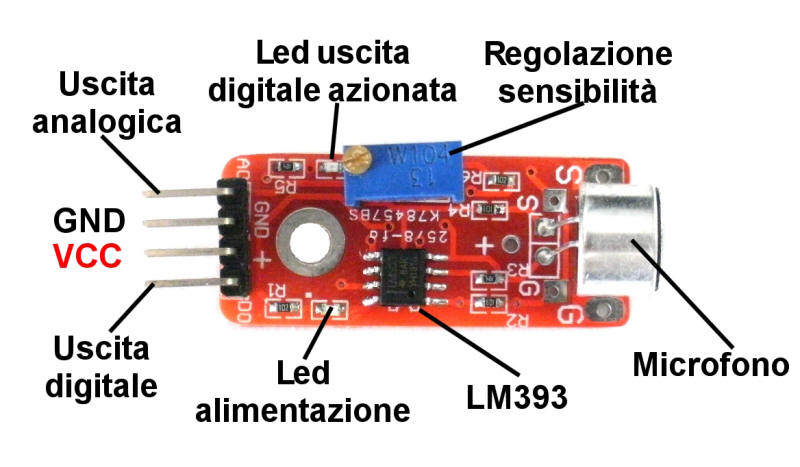
\includegraphics[width=0.4\textwidth]{imgs/KY-037-pin.jpg}
    \caption{Pinout del sensore KY-037.}
    \label{fig:KY-037}
\end{figure}

Il particolare, il circuito integrato LM393 presenta al suo interno due comparatori di tensione invertenti, i quali permettono di confrontare due tensioni e di generare un segnale in uscita in base al risultato di tale confronto.

\subsubsection{Circuito Elettronico del sensore KY-037}
Andando più nel dettaglio, possiamo fare riferimento al circuito mostrato in Figura \ref{fig:KY-037-circuit}.
Notiamo la presenta del microfono, contraddistinto dai terminali $S$ e $G$, dove il terminale $S$ è il terminale di segnale, mentre il terminale $G$ è il terminale di massa.
Il segnale audio rilevato viene fatto \textquotedblleft passare\textquotedblright\ attraverso la resistenza $R_3 = 150 \Omega$, giungendo ad un bivio (in gergo tecnico chiamato \textit{nodo}) dove una parte del segnale viene inviato al pin \lstinlinebg{A0} del sensore KY-037, mentre l'altra parte del segnale viene inviata all'ingresso invertente del primo comparatore di tensione presente nel circuito integrato LM393.
L'ingresso non invertente viene collegato al partitore di tensione formato dalle resistenze $R_2 = R_6 = 100 \text{k\Omega}$.

\begin{figure}[h]
    \centering
    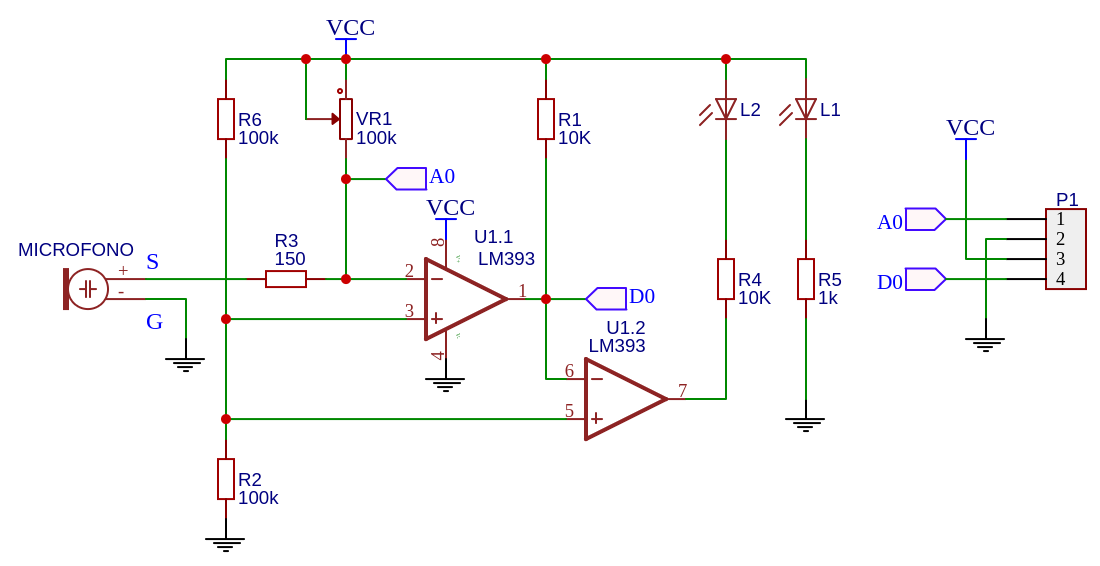
\includegraphics[width=0.75\textwidth]{imgs/circuito-ky037.png}
    \caption{Circuito elettronico del sensore KY-037.}
    \label{fig:KY-037-circuit}
\end{figure}

Si noti, inoltre, che il primo comparatore lavora unicamente con una tensione di alimentazione positiva ($V_{cc}$) perchè la tensione di alimentazione negativa ($-V_{cc}$) è collegata a massa.

Valgono, pertanto, le seguenti relazioni:

\begin{equation}
    V_{cc} = 5 \text{V}, \quad -V_{cc} = 0 \text{V} \nonumber
\end{equation}

Per quanto riuarda il comparatore di tensione, si tratta di un circuito elettronico che ha due ingressi, uno invertente e uno non invertente, un'uscita e due alimentazioni, come mostrato in Figura \ref{fig:comparatore_invertente}.

\begin{figure}[h]
    \centering
    \begin{tikzpicture}
        \begin{scope}[xshift=-4cm]
            \draw (0,0) node[op amp, scale=1.0] (opamp) {};
            \draw (opamp.-) to[short, -] ++(-1,0) node[left] {$v_{\text{in}}$};
            \draw (opamp.+) to[short, -] ++(-1,0) node[left] {$V_{\text{ref}}$};
            \draw (opamp.up) -- ++(0,.5) node[above] {$+V_{cc}$};
            \draw (opamp.down) -- ++(0,-.5) node[below] {$-V_{cc}$};
            \draw (opamp.out) -- ++(1,0) node[right] {$v_o$};
        \end{scope}
    \end{tikzpicture}
    \caption{Comparatore di tensione invertente.}
    \label{fig:comparatore_invertente}
\end{figure}

Il funzionamento del comparatore è molto semplice.
Si definiscono due tensioni di riferimento, $V_{\text{ref}}$ all'ingresso non invertente e $v_{\text{in}}$ all'ingresso invertente, dove $V_{\text{ref}}$ è la tensione di riferimento e $v_{\text{in}}$ è la tensione in ingresso.
Si definisce, inoltre, la tensione di saturazione dell'uscita del comparatore come $\pm V_{\text{sat}}$ che risulta essere sempre più piccola della tensione di alimentazione $\pm V_{cc}$.
Se la tensione in ingresso $v_{\text{in}}$ è minore della tensione di riferimento $V_{\text{ref}}$, l'uscita del comparatore sarà $+V_{\text{sat}}$.
Al contrario, se la tensione in ingresso $v_{\text{in}}$ è maggiore della tensione di riferimento $V_{\text{ref}}$, l'uscita del comparatore sarà $-V_{\text{sat}}$.
In formule otteniamo:

\begin{equation}
    v_{o} = \begin{cases}
        +V_{\text{sat}} & \text{se } v_{\text{in}} < V_{\text{ref}} \\
        -V_{\text{sat}} & \text{se } v_{\text{in}} > V_{\text{ref}}
    \end{cases} \label{eq:comparatore}
\end{equation}

La seguente Figura \ref{fig:waveforms}, mostra come il comparatore invertente effettui una vera e propria conversione analogico-digitale del segnale in ingresso $v_{\text{in}}$ in un segnale digitale $v_{o}$.

\begin{figure}[h]
    \centering
    \begin{tikzpicture}[>=latex, scale=0.8] % Aggiunta di scale per aumentare proporzioni
        % Griglia superiore estesa
        \draw[help lines, color=gray!30, dashed]
        (0,-2) grid (10,2);
        
        % Assi superiori estesi
        \draw[->,thick] (-0.5,0) -- (10.5,0) node[right] {$t$};
        \draw[->,thick] (0,-2.5) -- (0,2.5) node[above] {};
        
        % Linea Vref con etichetta spostata a sinistra
        \draw[dashed,black,thick] (-0.5,1) -- (10.5,1);
        \node[black,anchor=east] at (-0.5,1) {$V_{\text{ref}}$};
        
        % Sinusoide estesa
        \draw[black,thick,smooth] plot[domain=0:10,samples=300] 
        (\x,{1.5*sin(2*\x*57.296)});
        
        % Punti di intersezione aggiornati
        \foreach \x in {0.37,1.21,3.51,4.35,6.65,7.5,9.8} {
            \fill[black] (\x,1) circle (2pt);
        }
        
        % Etichetta della sinusoide (v_in) spostata a sinistra
        \node[black] at (-0.7,2.5) {$v_{\text{in}}(t)$};
        
        % Assi inferiori
        \begin{scope}[yshift=-4cm]
            % Griglia inferiore estesa
            \draw[help lines, color=gray!30, dashed]
            (0,-2) grid (10,2);
            
            \draw[->,thick] (-0.5,0) -- (10.5,0) node[right] {$t$};
            \draw[->,thick] (0,-2.5) -- (0,2.5) node[above] {};
            
            % Etichette asse Y inferiore con +/-Vsat a sinistra
            \draw (0.1,1.5) -- (-0.1,1.5) node[left] {$+V_{\text{sat}}$};
            \draw (0.1,-1.5) -- (-0.1,-1.5) node[left] {$-V_{\text{sat}}$};
            
            % Onda quadra corretta
            \draw[black,ultra thick] 
            (0,1.5) -- (0.37,1.5) -- (0.37,-1.5) -- (1.21,-1.5) --
            (1.21,1.5) -- (3.51,1.5) -- (3.51,-1.5) -- (4.35,-1.5) --
            (4.35,1.5) -- (6.65,1.5) -- (6.65,-1.5) -- (7.5,-1.5) --
            (7.5,1.5) -- (9.8,1.5) -- (9.8,-1.5) -- (10,-1.5); % Modificato per non terminare con una retta
            
            % Etichetta onda quadra (v_o) spostata a sinistra
            \node[black] at (-0.7,2.5) {$v_o(t)$};
        \end{scope}
        
        % Linee tratteggiate di corrispondenza aggiornate
        \foreach \x in {0.37,1.21,3.51,4.35,6.65,7.5,9.8} {
            \draw[black,dashed,thick] (\x,1) -- (\x,-2);
            \draw[black,dashed,thick] (\x,-2) -- (\x,-4.5);
        }
        
    \end{tikzpicture}
    \caption{Forme d'onda del comparatore invertente.}
    \label{fig:waveforms}
\end{figure}

Va specificato che le relazioni \eqref{eq:comparatore} valgono per un comparatore di tensione invertente avente due tensioni di alimentazione $\pm V_{cc} \neq 0$.
Diversamente, nel caso del sensore KY-037, il comparatore di tensione invertente ha la tensione di alimentazione positiva $+V_{cc} \neq 0$ e la tensione di alimentazione negativa $-V_{cc} = 0 \text{V}$.
Pertanto, le suddette relazioni si possono riscrivere come segue:

\begin{equation}
    v_{o} = \begin{cases}
        V_{\text{sat}} & \text{se } v_{\text{in}} < V_{\text{ref}} \\
        0  & \text{se } v_{\text{in}} > V_{\text{ref}}
    \end{cases} \nonumber
\end{equation}

Se immaginiamo di considerare la tensione di saturazione $V_{\text{sat}}$ come un livello logico alto e la tensione $0$ come un livello logico basso, possiamo ottenere i grafici mostrati in Figura \ref{fig:waveforms} con l'uscita $v_o$ traslata di $V_{\text{sat}}$ verso l'alto, quindi una vera e propria onda digitale con valori logici $0$ e $V_{\text{sat}}$, come mostrato in Figura \ref{fig:waveforms_translated}.

È importante sottolineare che il pin \lstinlinebg{A0}, corrispondente al segnale $v_{\text{in}}$, viene inviato al sistema digitale.
Pertanto, il segnale $v_{o}$ rappresenta il segnale audio digitalizzato che rimane all'interno del sensore KY-037 e viene utilizzato, insieme al diodo led $L_2$, per indicare la presenza o l'assenza di un segnale audio.

Ora, facendo riferimento alla Figura \ref{fig:KY-037-circuit}, quando la tensione sul pin 2 (del primo comparatore) proveniente dal ramo formato dal microfono e regolata dal potenziometro $V_{R_1}$ da $10 \text{k\Omega}$, è inferiore a quella presente sul pin 3 (del primo comparatore), si avrà in uscita, sul pin 1, un segnale $V_{\text{sat}}$.
Qualora la tensione sul pin 2 fosse maggiore, si otterrà un livello $0$.

Il secondo comparatore dell'integrato LM393 viene utilizzato per pilotare l'accensione del diodo led $L_2$, il quale segnala la rilevazione di un suono che supera la soglia impostata.
L'accensione del diodo led $L_1$, invece, indicherà la presenza della tensione di alimentazione, visto che il sensore è collegato a $V_{cc}$ e a massa tramite la resistenza $R_5 = 1 \text{k\Omega}$.

\begin{figure}[h]
    \centering
    \begin{tikzpicture}[>=latex, scale=0.8] % Aggiunta di scale per aumentare proporzioni
        % Griglia superiore estesa
        \draw[help lines, color=gray!30, dashed]
        (0,-2) grid (10,2);
        
        % Assi superiori estesi
        \draw[->,thick] (-0.5,0) -- (10.5,0) node[right] {$t$};
        \draw[->,thick] (0,-2.5) -- (0,2.5) node[above] {};
        
        % Linea Vref con etichetta spostata a sinistra
        \draw[dashed,black,thick] (-0.5,1) -- (10.5,1);
        \node[black,anchor=east] at (-0.5,1) {$V_{\text{ref}}$};
        
        % Sinusoide estesa
        \draw[black,thick,smooth] plot[domain=0:10,samples=300] 
        (\x,{1.5*sin(2*\x*57.296)});
        
        % Punti di intersezione aggiornati
        \foreach \x in {0.37,1.21,3.51,4.35,6.65,7.5,9.8} {
            \fill[black] (\x,1) circle (2pt);
        }
        
        % Etichetta della sinusoide (v_in) spostata a sinistra
        \node[black] at (-0.7,2.5) {$v_{\text{in}}(t)$};
        
        % Assi inferiori
        \begin{scope}[yshift=-6cm] % Spostamento più grande per accomodare raddoppio
            % Griglia inferiore estesa
            \draw[help lines, color=gray!30, dashed]
            (0,0) grid (10,4);
            
            \draw[->,thick] (-0.5,0) -- (10.5,0) node[right] {$t$};
            \draw[->,thick] (0,-0.5) -- (0,4.5) node[above] {};
            
            % Etichette asse Y inferiore con 0 e V_sat
            \draw (0.1,3) -- (-0.1,3) node[left] {$V_{\text{sat}}$};
            
            % Onda quadra raddoppiata
            \draw[black,ultra thick] 
            (0,3) -- (0.37,3) -- (0.37,0) -- (1.21,0) --
            (1.21,3) -- (3.51,3) -- (3.51,0) -- (4.35,0) --
            (4.35,3) -- (6.65,3) -- (6.65,0) -- (7.5,0) --
            (7.5,3) -- (9.8,3) -- (9.8,0) -- (10,0); % Modificato per raddoppiare ampiezza
            
            % Etichetta onda quadra (v_o) spostata a sinistra
            \node[black] at (-0.7,4.5) {$v_o(t)$};
        \end{scope}
        
        % Linee tratteggiate di corrispondenza aggiornate
        \foreach \x in {0.37,1.21,3.51,4.35,6.65,7.5,9.8} {
            \draw[black,dashed,thick] (\x,1) -- (\x,0);
            \draw[black,dashed,thick] (\x,0) -- (\x,-4.5);
        }
        
    \end{tikzpicture}
    \caption{Forme d'onda del comparatore invertente traslate.}
    \label{fig:waveforms_translated}
\end{figure}

È necessario, inoltre, regolare preventivamente il potenziometro $V_{R_1}$ per ottenere il segnale $V_{\text{sat}}$ solo qualore il rumore superi la soglia desiderata.
La taratura è relativamente semplice, facilitata dalla presenza del diodo led $L_2$: dopo aver agito in senso orario sulla vite del potenziometro fino allo spegnimento del diodo led $L_2$, se si emette un suono ed il led si accende nuovamente, significa che il sensore è in grado di riconoscere il livello di rumore e quindi di produrre un segnale $V_{\text{sat}}$ in uscita.

\subsection{Sistema digitale}
Alcuni anni fa, il mondo dell'IoT Embedded ha subito una rivoluzione ad opera della scheda ESP8266, microcontrollore programmabile, abilitato al Wi-Fi ed in grado di monitorare e controllare sensori da qualsiasi parte del mondo.
A seguito dello straordinario successo ottenuto, Espressif, l'azienda di semiconduttori che ha ideato tale scheda, ha rilasciato un perfetto aggiornamento potenziato: l'ESP32, che incorpora non solo il Wi-Fi ma anche il Bluetooth 4.0 (BLE/Bluetooth Smart), così da renderla la scheda ideale per qualsiasi applicazione Internet of Things.
Tra le numerose schede della famiglia ESP32 quella utilizzata per la realizzazione di questo progetto è la scheda ESP32 DevKit V1.

\subsubsection{Modulo ESP-WROOM-32}
La scheda ESP32 DevKit V1 è dotata del modulo ESP-WROOM-32, che contiene il microprocessore Tensilica Xtensar Dual-Core a $32$ bit LX6.
Questo processore è simile a quello utilizzato nell'ESP8266, ma ha due core CPU (che possono essere controllati individualmente).
La frequenza di clock è regolabile da $80 \text{Hz}$ a $240 \text{MHz}$ e può funzionare fino a $600 \text{DMIPS}$ (Dhrystone Million Instructions Per Second).
La scheda presenta anche $448 \text{KB}$ di ROM, $520 \text{KB}$ di SRAM e $4 \text{MB}$ di memoria Flash (per programmi e archiviazione dati) sufficienti per gestire le lunghe stringhe che compongono le pagine Web o i dati JSON/XML.
L'ESP32 incorpora un ricetrasmettitore Wi-Fi 802.11b/g/n HT40, che consente la connessione a reti Wi-Fi per accedere a Internet (Station mode) o per creare la propria rete wireless Wi-Fi (Soft access point mode) a cui possono connettersi altri dispositivi.

\begin{figure}[h]
    \centering
    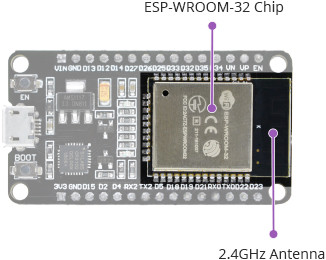
\includegraphics[width=0.35\textwidth]{imgs/ESP32-Hardware-Specifications-ESP-WROOM-32-Chip.jpg}
    \caption{Modulo ESP-WROOM-32}
    \label{fig:ESP-WROOM-32}
\end{figure}

L'ESP32 supporta anche il Wi-Fi Direct, che è una buona opzione per le connessioni peer-to-peer che non richiedono un access point.
Il Wi-Fi Direct è più semplice da configurare e offre velocità di trasferimento dati molto più elevate rispetto al Bluetooth.
La scheda supporta sia il Bluetooth 4.0 (BLE/Bluetooth Smart) che il Bluetooth Classic (BT), il che la rende ancora più versatile.

\subsubsection{Alimentazione elettrica}
Poiché l'intervallo di tensione operativa dell'ESP32 è compreso tra $2.2 \text{V}$ e $3.6 \text{V}$, la scheda include un regolatore di tensione LDO per mantenere la tensione stabile a $3.3 \text{V}$, in modo da fornire fino a $600 \text{mA}$ di corrente.

\begin{figure}[h]
    \centering
    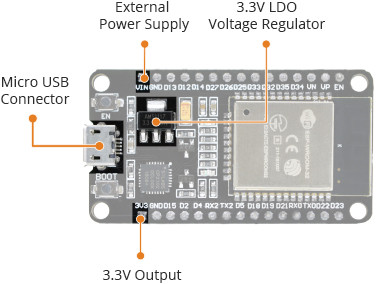
\includegraphics[width=0.35\textwidth]{imgs/ESP32-Hardware-Specifications-Power-Supply.jpg}
    \caption{Alimentazione elettrica e regolatore di tensione LDO}
    \label{fig:ESP32-LDO}
\end{figure}

L'uscita del regolatore da $3.3 \text{V}$ viene distribuita al pin della scheda etichettato con \lstinlinebg{3V3}, che può essere utilizzato per alimentare circuiti esterni.
Generalmente viene alimentata dal connettore Micro USB integrato, ma se si dispone di un alimentatore da $5 \text{V}$, è possibile utilizzare il pin etichettato con \lstinlinebg{VIN} per alimentare direttamente l'ESP32 e le sue periferiche.
Quest'ultimo metodo è quello che è stato utilizzato in questo progetto per l'alimentazione del display OLED e del sensore KY-037.

% TODO:
\subsubsection{Periferiche e I/O}
Sebbene l'ESP32 abbia in totale $30$ pin, solo $25$ di essi sono GPIO (General Purpose Input Output) e quindi accessibili tramite i rispettivi pin che si trovano sulla scheda.
La piedinatura è la seguente:

\begin{figure}[h]
    \centering
    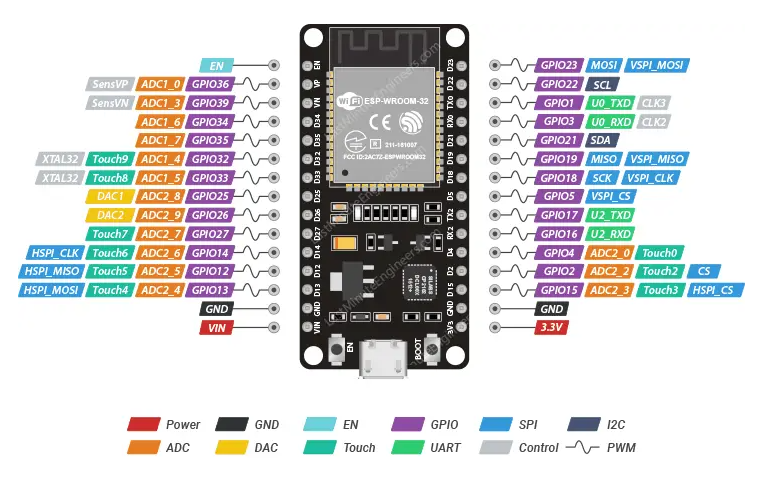
\includegraphics[width=0.65\textwidth]{imgs/pinout.png}
    \caption{Pinout della scheda}
    \label{fig:ESP32-pinout}
\end{figure}

A questi pin può essere assegnata una varietà di compiti, tra cui $15$ canali di ADC a $12$ bit con intervalli selezionabili di $[0, 1] \text{V}$, $[0, 1.4] \text{V}$, $[0, 2] \text{V}$ o $[0, 4] \text{V}$, due interfacce UART (Universal Asiynchronous Receiver-Transmitter) con controllo di flusso e supporto IrDA (Infrared Data Association), $25$ pin PWM (Pulse Width Modulation) per controllare la velocità di un motore o la luminosità di un diodo led, due DAC a $8$ bit per generare tensioni analogiche, tre interfacce SPI (Serial Peripheral Interface), un'interfaccia I2C (Inter-Integrated Circuit) per collegare vari sensori e periferiche ed infine due interfacce I2S\footnote{Il protocollo I2S è molto complesso e richiede il framework nativo di Espressif nella configurazione dell'ecosistema PlatformIO. In questo progetto si è scelto di utilizzare il framework di Arduino per garantire maggiore compatibilità con entrambe le schede. Per maggiorni informazioni è possibile consultare la sezione \ref{sec:future}.} per collegare microfoni e altoparlanti, ed infine $9$ Touch Pads GPIO con rilevamento tattile capacitivo.

\begin{figure}[h]
    \centering
    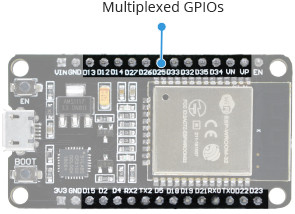
\includegraphics[width=0.35\textwidth]{imgs/ESP32-Hardware-Specifications-Multiplexed-GPIO-pins.jpg}
    \caption{Periferiche e I/O}
    \label{fig:ESP32-I/O}
\end{figure}

In particolare la funzione multiplexing, dei pin dell'ESP32, consente a più periferiche di condividere un singolo pin GPIO, infatti, un singolo pin GPIO può fungere da ingresso ADC, uscita DAC o Touch Pad.
Infine i pin \lstinlinebg{GPIO34}, \lstinlinebg{GPIO35}, \lstinlinebg{GPIO36(VP)} e \lstinlinebg{GPIO39(VN)} non possono essere configurati come uscite.
Possono essere utilizzati come ingressi digitali o analogici o per altri scopi.
Inoltre non dispongono di resistori pull-up e pull-down interni, a differenza degli altri pin GPIO.

\subsubsection{Interruttori e indicatori LED}
Sono presenti due pulsanti sulla scheda ESP32.
Il pulsante Reset, etichettato \lstinlinebg{EN}, viene utilizzato per ripristinare il chip ESP32.
L'altro pulsante è il pulsante Boot, che viene utilizzato per scaricare nuovi software o programmi.

\begin{figure}[h]
    \centering
    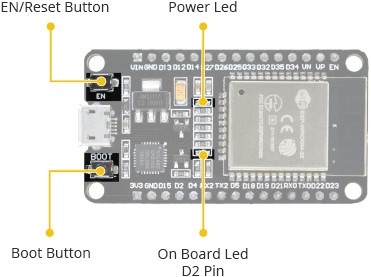
\includegraphics[width=0.35\textwidth]{imgs/ESP32-Hardware-Specifications-Reset-Boot-Buttons-LED-Indicators.jpg}
    \caption{Interruttori e indicatori LED}
    \label{fig:ESP32-LED}
\end{figure}

La scheda include anche due indicatori led. Il diodo led rosso indica che la scheda è accesa, mentre il diodo led blu è programmabile ed è collegato al pin \lstinlinebg{D2} della scheda.

\subsubsection{Comunicazione seriale}
La scheda include il controller bridge USB-to-UART CP2102 di Silicon Labs, che converte i segnali USB in seriali e consente di programmare il chip ESP32.

\begin{figure}[h]
    \centering
    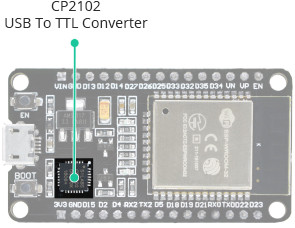
\includegraphics[width=0.3\textwidth]{imgs/ESP32-Hardware-Specifications-USB-to-TTL-Converter.jpg}
    \caption{Comunicazione seriale}
    \label{fig:ESP32-serial}
\end{figure}

\subsection{Display OLED}
I display OLED sono disponibili in una vasta gamma di dimensioni (per esempio $128 \times 64$ o $128 \times 32$) e colori (per esempio OLED bianco, blu e bicolore).
Alcuni display OLED hanno un'interfaccia I2C, mentre altri hanno un'interfaccia SPI.
Una cosa che hanno tutti in comune, tuttavia, è la presenza di un potente controller driver OLED CMOS a chip singolo: l'SSD1306.
Quest'ultimo gestisce tutto il buffering della RAM.
Il display OLED che è stato utilizzato per il progetto ha dimensioni $128 \times 64$ ed utilizza un'interfaccia I2C, rispettivamente con collegamenti rispettivamente ai pin SCL (\lstinlinebg{GPIO22}) e SDA (\lstinlinebg{GPIO21}), ed è molto simile a quello mostrato in Figura \ref{fig:OLED}.

\begin{figure}[h]
    \centering
    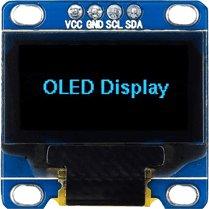
\includegraphics[width=0.15\textwidth]{imgs/128x64-Blue-I2C-OLED-Display.jpg}
    \caption{Display OLED}
    \label{fig:OLED}
\end{figure}

Un display OLED, a differenza di un display LCD a caratteri, non richiede retroilluminazione perché genera luce propria.
Ciò spiega l'elevato contrasto del display, l'angolo di visione estremamente ampio e la capacità di visualizzare livelli di nero profondo.
L'assenza di retroilluminazione riduce significativamente il consumo energetico.
Il display utilizza in media circa $20 \text{mA}$, anche se questo varia a seconda della quantità di display illuminato.
Il controller SSD1306 lavora tra $1.65 \text{V}$ e $3.3 \text{V}$, mentre il pannello OLED richiede una tensione di alimentazione compresa tra $7 \text{V}$ e $15 \text{V}$.
Tutti i requisiti di alimentazione sono soddisfatti dal circuito interno della pompa di carica\footnote{La pompa di carica è un circuito elettronico che usa dei condensatori per immagazzinare energia in maniera da ottenere delle sorgenti con tensioni più elevate o più basse di quelle disponibili dall'alimentazione.}.
Ciò rende possibile collegare il display OLED alla scheda ESP32 o a qualsiasi altro microcontrollore logico da $5 \text{V}$ senza utilizzare un convertitore di livello logico.

\subsubsection{Mappatura della memoria}
Per controllare il display è fondamentale comprendere la mappatura della memoria.
Indipendentemente dalle dimensioni\footnote{Ogni modulo contiene $\text{M} = 1 \text{KB}$ di RAM. Il modulo OLED $128 \times 64$ visualizza l'intero contenuto di $\text{M} = 1 \text{KB}$ di RAM (tutte le $8$ pagine), mentre il modulo OLED $128 \times 32$ visualizza solo metà della RAM (le prime $4$ pagine).} del display OLED, il driver SSD1306 include una RAM di dati di visualizzazione grafica (GDDRAM) da $1 \text{KB}$ che memorizza il pattern di bit da visualizzare sullo schermo.
Quest'area di memoria $\text{M} = 1 \text{KB}$ è divisa in $p = 8$ pagine (da $0$ a $7$).
Ogni pagina ha $s = 128$ colonne o segmenti (blocco da $0$ a $127$).
Inoltre, ciascuna colonna può memorizzare $n = 8$ bit di dati (da $0$ a $7$).
Pertanto è facile dimostrare che la memoria $\text{M}$ vale:

\begin{equation}
    \text{M} = p \cdot s \cdot n = 8 \cdot 128 \cdot 8 = 8192 \text{ bit} = 1024 \text{ byte} = 1 \text{KB} \nonumber
\end{equation}

L'intera memoria da $1 \text{KB}$, incluse pagine, segmenti e dati, è evidenziata in Figura \ref{fig:memory-mapping}.

\begin{figure}[h]
    \centering
    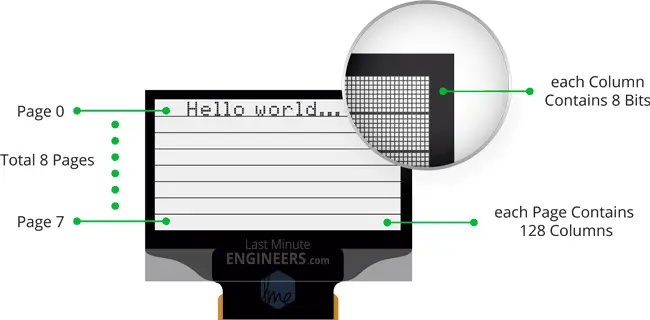
\includegraphics[width=0.4\textwidth]{imgs/1KB-128x64-OLED-Display-RAM-Memory-Map.png}
    \caption{Mappatura della memoria $\text{M} = 1 \text{KB}$}
    \label{fig:memory-mapping}
\end{figure}

In particolare, ogni bit rappresenta un singolo pixel sullo schermo che può essere attivato o disattivato direttamente dal codice.

\subsection{Schema di montaggio finale}
In conclusione, l'intero sistema, dal punto di vista hardware, è composto da un microfono KY-037, un display OLED $128 \times 64$ e una scheda ESP32 DevKit V1.
Pertanto collegando adeguatamente i vari componenti, come mostrato in Figura \ref{fig:final-schematic}, è possibile realizzare un analizzatore di spettro audio real-time.

\begin{figure}[h]
    \centering
    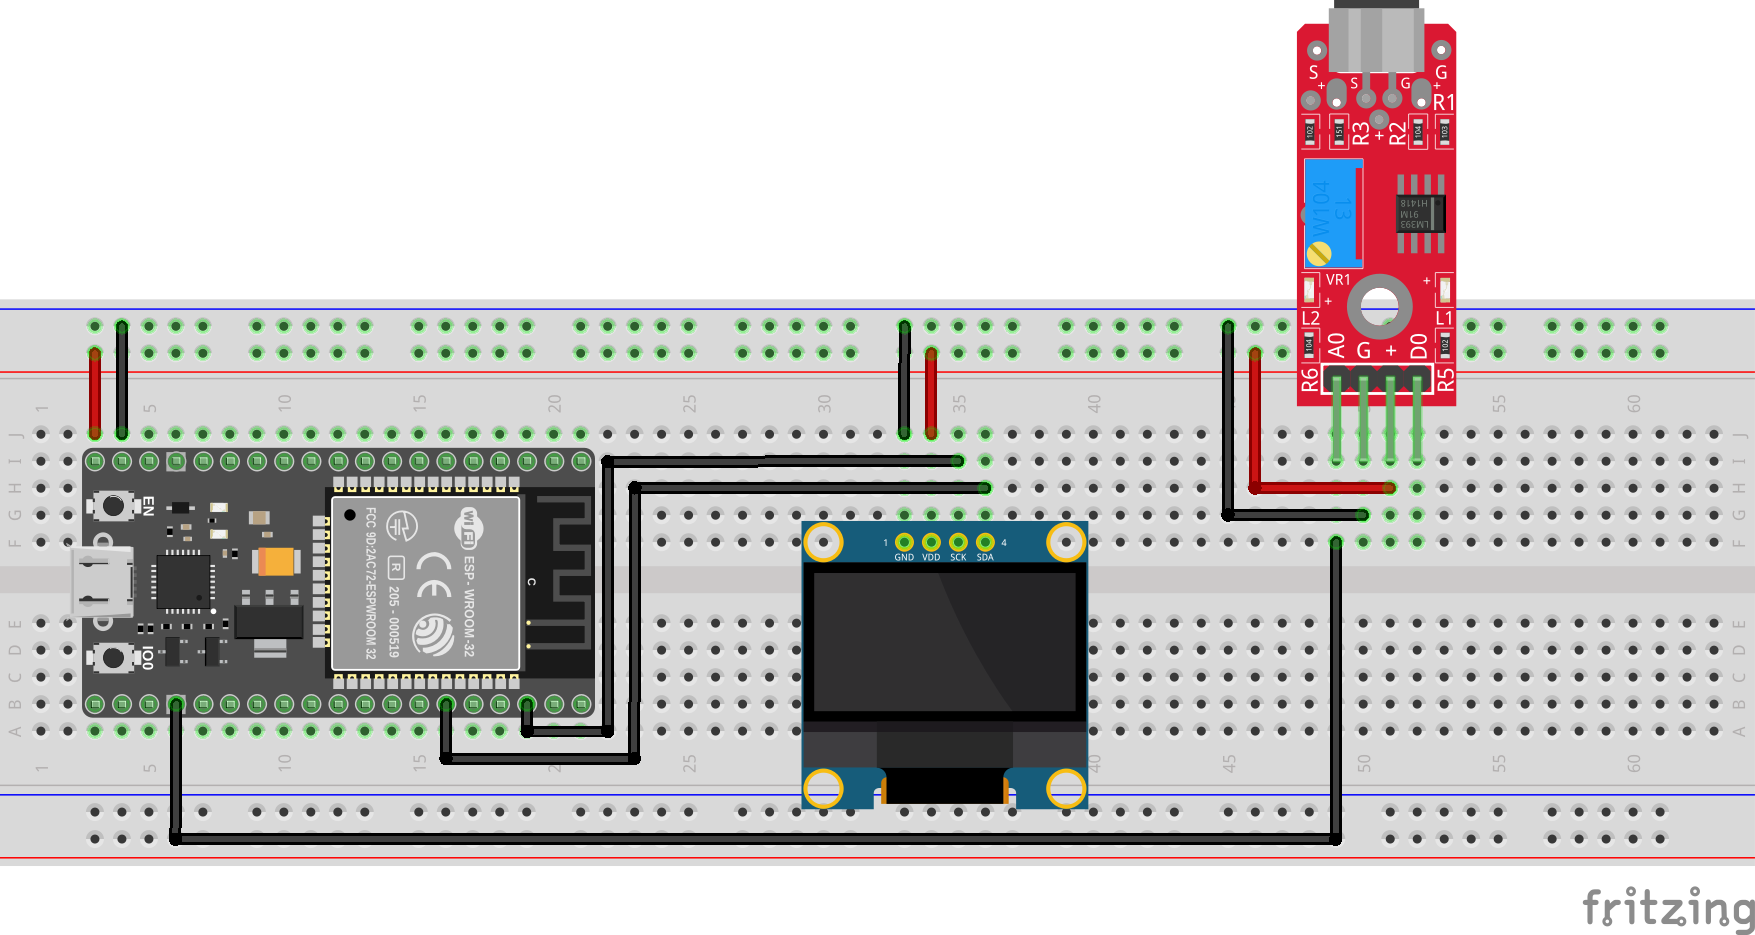
\includegraphics[width=0.75\textwidth]{imgs/schema-di-montaggio.png}
    \caption{Schema di montaggio finale}
    \label{fig:final-schematic}
\end{figure}

Tuttavia occorre finalizzare ancora il progetto con il firmware, che permetterà di acquisire il segnale audio dal sensore KY-037, di calcolare la DFT del segnale e di visualizzare lo spettro del segnale sul display OLED.

\section{Progettazione del firmware}\label{sec:code}

\subsection{Introduzione}
Per realizzare il firmware del progetto è stato utilizzato il framework di Arduino, che permette di programmare la scheda ESP32 DevKit V1 utilizzando il linguaggio di programmazione C\texttt{++}.
A tale scopo si è utilizzato l'ecosistema open-source di PlatformIO, che permette di programmare microcontrollori e microprocessori in modo professionale, fornendo un ambiente di sviluppo integrato (IDE) per la scrittura del codice, la compilazione e il caricamento del firmware sul microcontrollore.
In questa sezione si discutono le scelte progettuali relative al firmware del progetto, con particolare attenzione all'acquisizione del segnale audio, al calcolo della DFT e alla visualizzazione dello spettro del segnale.
Alcune parti di codice sono già state discusse nelle sezioni precedenti, pertanto si discuteranno solo le parti di codice più significative.

\subsection{Organizzazione del progetto}
Il progetto è organizzato in diverse cartelle e file, come mostrato in Figura \ref{fig:project-structure}.
In particolare la cartella \lstinlinebg{src/} contiene i file \lstinlinebg{main.cpp} e \lstinlinebg{fft.cpp} mentre la cartella \lstinlinebg{include/} contiene i file \lstinlinebg{fft.h} e \lstinlinebg{settings.h}.
Inoltre è presente anche il file \lstinlinebg{platformio.ini} che contiene le impostazioni del progetto relative al framework di Arduino, alla scheda ESP32 DevKit V1 e ad altre librerie esterne utilizzate nel progetto.

\begin{figure}[h]
    \centering
    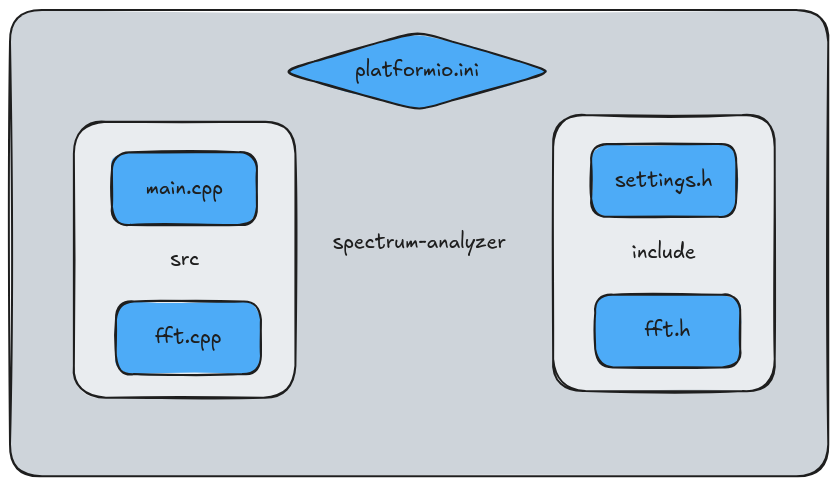
\includegraphics[width=0.6\textwidth]{imgs/project-structure.png}
    \caption{Struttura del progetto}
    \label{fig:project-structure}
\end{figure}

In particolare, per utilizzare il display OLED con la scheda ESP32, è necessario installare la libreria \lstinlinebg{Adafruit_SSD1306} e la libreria \lstinlinebg{Adafruit_GFX}.
Pertanto occorre modificare il file \lstinlinebg{platformio.ini} come mostrato di seguito:

\begin{lstlisting}[language=Python, keywords={platform, board, framework, lib_deps}]
[env:esp32doit-devkit-v1]
platform = espressif32
board = esp32doit-devkit-v1
framework = arduino
lib_deps = 
    adafruit/Adafruit SSD1306@^2.5.13
    adafruit/Adafruit GFX Library@^1.11.11
\end{lstlisting}

Ora, facendo riferimento alla Figura \ref{fig:project-structure}, il file \lstinlinebg{settings.h} contiene le impostazioni del progetto, come ad esempio la dimensione del display OLED e la frequenza di campionamento del segnale audio.
Vediamolo nel dettaglio:

\begin{lstlisting}[language=C++, keywords={constexpr, uint32_t, uint8_t, uint16_t}]
#pragma once

#include <Arduino.h>
#include <Wire.h>

// External Libraries
#include <Adafruit_GFX.h>
#include <Adafruit_SSD1306.h>

// Serial Communication Variables
constexpr uint32_t BAUD_RATE = 115200;
constexpr uint8_t ADC_RESOLUTION = 12;

// Audio Input Variables
constexpr uint8_t AUDIO_IN_PIN = 34;

// Adafruit OLED Display Variables
#define SCREEN_WIDTH   128
#define SCREEN_HEIGHT  64
#define OLED_RESET     4
#define SCREEN_ADDRESS 0x3C

// FFT Variables
constexpr uint16_t SAMPLE_RATE = 22050; // 22.05kHz (using Nyquist-Shannon Theorem)
constexpr uint16_t SAMPLES = 128;
constexpr uint8_t BAR_WIDTH = 2;
constexpr uint8_t BAR_SPACING = 2;
\end{lstlisting}

dove alcune variabili sono autoesplicative, come ad esempio la variabile \lstinlinebg{BAUD_RATE} che rappresenta la velocità di trasmissione dati seriale, la variabile \lstinlinebg{ADC_RESOLUTION} che rappresenta la risoluzione del convertitore analogico-digitale, la variabile \lstinlinebg{AUDIO_IN_PIN} che rappresenta il pin di ingresso del segnale audio, la variabile \lstinlinebg{SAMPLE_RATE} che rappresenta la frequenza di campionamento del segnale audio e la variabile \lstinlinebg{SAMPLES} che rappresenta il numero di campioni del segnale audio.
Altre variabili, come ad esempio la variabile \lstinlinebg{BAR_WIDTH} che rappresenta la larghezza delle barre dello spettro del segnale audio e la variabile \lstinlinebg{BAR_SPACING} che rappresenta lo spazio tra le barre dello spettro del segnale audio, sono state scelte in modo arbitrario per ottenere un risultato visivo gradevole.

In particolare, il display OLED ha $128$ colonne, è possibile visualizzare su di esso solo $128$ frequenze dello spettro del segnale audio.
Tuttavia, avendo definito le variabili \lstinlinebg{BAR_WIDTH} e \lstinlinebg{BAR_SPACING}, è possibile visualizzare un numero minore di frequenze (proprio perchè vengono aggiunti degli spazi vuoti, ossia delle colonne del display che non saranno mai accese).
Quindi è possibile calcolare il numero di frequenze visualizzate con la seguente formula:

\begin{equation}
    \text{Frequenze visualizzate} = \frac{\text{SCREEN WIDTH}}{\text{BAR WIDTH} + \text{BAR SPACING}} = \frac{128}{2 + 2} = 32 \text{ frequenze} \nonumber
\end{equation}

mentre la frequenza $f_b$ associata a ciascuna barra dello spettro è data dalla formula:

\begin{equation}
    f_b = \frac{f_s}{N} \cdot n \nonumber
\end{equation}

dove $f_s$ è la frequenza di campionamento, $N$ è il numero di campioni e $n$ rappresenta l'indice della barra che rappresenta una specifica banda di frequenze.

\noindent\\ \namedparagraph{Esempio.}{Per $n = 1$ si ha che la frequenza associata alla prima barra dello spettro è data da:
\begin{equation}
    f_b = \frac{22050}{128} \cdot 1 = 172.27 \text{Hz} \nonumber
\end{equation}
per $n = 2$ si ha che la frequenza associata alla seconda barra dello spettro è data da:
\begin{equation}
    f_b = \frac{22050}{128} \cdot 2 = 344.54 \text{Hz} \nonumber
\end{equation}
e così via fino a $n = 32$.}

\noindent\\ Continuiamo dunque con il file \lstinlinebg{main.cpp}, il cui contenuto è già stato spiegato in parte nella sezione \ref{sec:acquisition}.
Dunque, per chiarezza, riporto il codice completo del file \lstinlinebg{main.cpp}:

\begin{lstlisting}[language=C++, keywords={EngineFFT, const, uint8_t, if, for, void, Serial, begin, uint16_t, analogRead, println, uint32_t, micros, , pinMode, INPUT, displayInit, antiAliasingLowPassFilter, removeDC, windowing, fft, drawBigBars}]
#include "fft.h"

EngineFFT engine = EngineFFT();

const uint32_t interval = engine.samplingPeriod;
uint32_t lastUpdate = 0;

void setup() {
    engine.displayInit();
    pinMode(AUDIO_IN_PIN, INPUT);
    lastUpdate = micros();
}

void loop() {
    // Acquisition of audio samples
    if (micros() - lastUpdate >= interval) {
        lastUpdate = micros();
        for (uint8_t i = 0; i < SAMPLES; ++i) {
            uint16_t sample = analogRead(AUDIO_IN_PIN);
            engine.re[i] = engine.antiAliasingLowPassFilter(sample);
            engine.im[i] = 0.0;
        }

        // Real-Time FFT
        engine.removeDC();
        engine.windowing();
        engine.fft();
        engine.drawBigBars();
    }
}
\end{lstlisting}

come si può notare, il codice è diviso in due parti principali: la funzione \lstinlinebg{setup()} e la funzione \lstinlinebg{loop()}.
La funzione \lstinlinebg{setup()} inizializza il display OLED e imposta il pin \lstinlinebg{AUDIO_IN_PIN} come ingresso.
La funzione \lstinlinebg{loop()} acquisisce i campioni del segnale audio, calcola la DFT del segnale e visualizza lo spettro del segnale sul display OLED.
In particolare, è stata creata una classe \lstinlinebg{EngineFFT} che contiene tutti i metodi necessari per l'acquisizione del segnale audio, il calcolo della DFT e la visualizzazione dello spettro del segnale.
Quindi tutti i metodi della classe \lstinlinebg{EngineFFT} e la classe stessa, sono stati implementati nei file \lstinlinebg{fft.h} e \lstinlinebg{fft.cpp}.
Pertanto analizziamo nel dettaglio il contenuto del file \lstinlinebg{fft.h}:

\begin{lstlisting}[language=C++, keywords={class, public, private, uint16_t, uint8_t, float, constexpr, static, void, double, uint32_t, Adafruit_SSD1306, const}]
#pragma once

#include "settings.h"

class EngineFFT {
public:
    EngineFFT(void);
    void displayInit(uint32_t baudrate = BAUD_RATE);
    float antiAliasingLowPassFilter(uint16_t sample);
    void removeDC(void);
    void windowing(void);    // only Hann Window type
    void fft(void);          // only forward direction
    void drawBigBars(void);

    uint32_t samplingPeriod; // microseconds
    double re[SAMPLES];
    double im[SAMPLES];

private:
    void swap(double *x, double *y);
    void createMagnitudes(void);
    double getPeak(void);
    
    uint8_t levels;
    uint8_t fontSize;
    Adafruit_SSD1306 display;
    float lastFilteredValue;

    const float alpha = 0.15f;
    const uint16_t maxBars = SCREEN_WIDTH / (BAR_WIDTH + BAR_SPACING);
};
\end{lstlisting}

dove, poichè una buona parte dei metodi sono stati già discussi nelle sezioni \ref{sec:acquisition}, \ref{sec:filtering}, \ref{sec:windowing} e \ref{sec:fft}, in questa sezione, ci concentreremo unicamente sul costruttore della classe \lstinlinebg{EngineFFT} e sui metodi \lstinlinebg{displayInit()} e \lstinlinebg{drawBigBars()}.
In particolare, il costruttore della classe \lstinlinebg{EngineFFT} è definito come segue:

\begin{lstlisting}[language=C++, keywords={void, log2, uint32_t, this, round}]
EngineFFT::EngineFFT(void) {
    this->levels = log2(SAMPLES);
    this->samplingPeriod = round(1000000 * (1.0 / SAMPLE_RATE)); // T[us] = 1 / f => T * 10^(-6) = 1 / f => T = 10^6 / f
    this->fontSize = 1;
    this->lastFilteredValue = 0.0f;
}
\end{lstlisting}

dove vengono calcolati i livelli delle \textit{sub-DFT}, il periodo di campionamento del segnale audio ed inoltre viene inizializzata la dimensione del font del display OLED e il valore dell'ultimo campione filtrato.
Continuando, il metodo \lstinlinebg{displayInit()} che si occupa di inizializzare il display OLED, è definito come segue:

\begin{lstlisting}[language=C++, keywords={void, if, uint32_t, Serial, begin, Wire, Adafruit_SSD1306, SSD1306_SWITCHCAPVCC, clearDisplay, this, setTextColor, for, println}]
void EngineFFT::displayInit(uint32_t baudrate) {
    Serial.begin(baudrate);
    Wire.begin();
    
    this->display = Adafruit_SSD1306(SCREEN_WIDTH, SCREEN_HEIGHT, &Wire, OLED_RESET);
    if (!this->display.begin(SSD1306_SWITCHCAPVCC, SCREEN_ADDRESS)) {
        Serial.println(F("SSD1306 allocation failed"));
        for (;;);
    }
    this->display.setTextColor(WHITE);
    this->display.clearDisplay();
    this->display.display();
}
\end{lstlisting}

dove vengono inizializzati i pin di comunicazione seriale, il display OLED e il colore del testo.
Infine, il metodo \lstinlinebg{drawBigBars()} disegna le barre dello spettro del segnale sul display OLED e viene definito come segue:

\begin{lstlisting}[language=C++, keywords={void, uint8_t, uint16, for, uint16_t, this, sqrt, sq, double, return, fillRect, log, static_cast}]
void EngineFFT::createMagnitudes(void) {
    for (uint16_t i = 0; i < SAMPLES; ++i) {
        this->re[i] = sqrt(sq(this->re[i]) + sq(this->im[i]));
    }
}

double EngineFFT::getPeak(void) {
    double peak = 0.0;
    for (uint16_t i = 0; i < SAMPLES; ++i) {
        peak = (peak > this->re[i]) ? peak : this->re[i];
    }
    return peak;
}

void EngineFFT::drawBigBars(void) {
    this->createMagnitudes();
    double peak = this->getPeak();
        
    this->display.fillRect(0, 0, SCREEN_WIDTH, SCREEN_HEIGHT, BLACK);
    
    for (uint16_t i = 0; i < maxBars && i < SAMPLES; ++i) {
        double magnitude = this->re[i];
        double logMagnitude = magnitude > 0.0 ? log(magnitude + 1.0) : 0.0;
        double normalizedHeight = (logMagnitude / log(peak + 1.0)) * SCREEN_HEIGHT;
        uint16_t barHeight = static_cast<uint16_t>(normalizedHeight);
    
        uint16_t x = i * (BAR_WIDTH + BAR_SPACING);
        uint16_t y = SCREEN_HEIGHT - barHeight;
    
        this->display.fillRect(x, y, BAR_WIDTH, barHeight, WHITE);
    }
    
    this->display.display();
}
\end{lstlisting}

dove sono riportati anche i metodi \lstinlinebg{createMagnitudes()} e \lstinlinebg{getPeak()} che vengono utilizzati per calcolare le magnitudini e il picco dello spettro del segnale.
In particolare, la funzione \lstinlinebg{drawBigBars()} disegna le barre dello spettro del segnale sul display OLED, calcolando la magnitudine normalizzata di ciascuna barra e disegnando la barra sul display.
Per maggiori informazioni riguardo al codice sorgente del progetto e al funzionamento pratico è possibile consultare il repository GitHub del progetto all'indirizzo \url{https://github.com/AntonioBerna/spectrum-analyzer}.

\section{Conclusioni}\label{sec:future}
Il progetto dell'analizzatore di spettro audio rappresenta un esempio concreto di come sia possibile coniugare conoscenze teoriche e capacità pratiche per sviluppare uno strumento versatile e innovativo.
Questo lavoro ha offerto l'opportunità di esplorare a fondo l'elaborazione digitale dei segnali, l'ottimizzazione delle risorse hardware e software, e la progettazione di un sistema in grado di operare in tempo reale.
Le funzionalità attualmente implementate costituiscono una solida base per futuri sviluppi, che potrebbero ampliare le possibilità di utilizzo del dispositivo.
Alcune delle principali estensioni individuate includono:

\begin{itemize}
    \item L'adozione del protocollo I2S, per migliorare la qualità e la fedeltà dell'acquisizione del segnale audio.
    \item L'integrazione di una scheda microSD, per memorizzare tracce audio e consentire analisi successive con il dispositivo stesso o altri strumenti.
    \item L'utilizzo di un microfono MEMS, che semplificherebbe l'acquisizione audio diretta, garantendo al contempo compattezza e precisione.
    \item L'implementazione di un display TFT a colori, per migliorare la chiarezza e l'intuitività della rappresentazione visiva dello spettro audio.
\end{itemize}

Questi miglioramenti, oltre a rafforzare l'efficacia e la fruibilità del sistema, aprono la strada a molteplici applicazioni pratiche, dall'uso educativo e didattico alla progettazione audio professionale.
Inoltre, consentirebbero di soddisfare esigenze sempre più complesse, mantenendo al contempo una struttura compatta e accessibile.

In sintesi, il progetto ha dimostrato il valore di un approccio integrato alla progettazione di strumenti elettronici, combinando creatività, ricerca e soluzioni tecniche efficaci.
Le estensioni prospettate rappresentano un naturale completamento di questo lavoro, permettendo di rendere il dispositivo un punto di riferimento per applicazioni pratiche nel campo dell'analisi audio.

\end{document}